\chapter{C++ Classes in the Library}\label{ch-classes}
\thispagestyle{headings}
\markboth{Chapter \ref{ch-classes}: C++ Classes in the Library}{Chapter \ref{ch-classes}: C++ Classes in the Library}



QUESO is is a parallel object-oriented statistical library dedicated to the research of   statistically robust, scalable, load balanced, and fault-tolerant mathematical algorithms for the  quantification of uncertainty in realistic computational models and predictions related to natural and engineering systems.



Classes in QUESO can be divided in four main groups: core, templated basic, templated statistical and miscellaneous.
The classed that handle environment (and options), vector and matrix classes are considered \textit{core} classes. Classes implementing vector sets and subsets, vector spaces,  scalar functions, vector functions, scalar sequences and vector sequences are \textit{templated basic} classes; they are necessary for the definition and description of other entities, such as RVs, Bayesian solutions of IPs, sampling algorithms and chains.  Vector realizer, vector RV, statistical IP (and options), MH solver (and options), statistical FP (and options), MC solver (and options) and sequence statistical options are part of \textit{templated statistical} classes. And finally, the \textit{miscellaneous} classes consist of C and FORTRAN interfaces.



%The QUESO-MCMC Tool currently implements the DRAM algorithm \cite{HaLaMiSa06} for the generation of a Markov chain.
%Section \ref{sc-gmc-eight-steps} explains how to develop your own application using the DRAM capabilities of the QUESO-MCMC Tool, while
%Section \ref{sc-gmc-dram-output} describes the output information generated by the toolkit and
%Sections
%\ref{sc-gmc-dram-normal-ex},
%\ref{sc-gmc-dram-chem-ex} and
%\ref{sc-gmc-dram-algae-ex}
%describe the three examples available,
%all of them also available in \cite{mcmctool}.

%The chapter ends at Section \ref{sc-gmc-planned-features} with a brief list of planned features for next toolkit versions w.r.t. Markov Chain Monte Carlo methods.

\section{Core Classes}


QUESO core classes are the classes responsible for handling the environment (and options), vector
and matrix operations. They are described in the following sections.

% 
% \begin{description}
% \item[ core:] environment (and options), vector, matrix;
% 
% \item[ templated basic:] vector sets (and subsets, vector spaces),  scalar function, vector function, scalar sequence, vector sequence;
% 
% The templated basic classes are necessary for the definition and description of other entities, such as RVs, Bayesian solutions of IPs, sampling algorithms and chains.
% 
% %\item Vector sets, subsets and spaces (see Figure \ref{fig-vector-space-subset-classes}),
% %\item Scalar function (see Figure \ref{fig-scalar-function-class}),
% %\item Vector function (see Figure \ref{fig-vector-function-class}),
% %\item Scalar sequence (see Figure \ref{fig-scalar-sequence-class}), and
% %\item Vector sequence (see Figure \ref{fig-vector-sequence-class}).
% 
% \item[ templated statistical:] vector realizer, vector RV, statistical IP (and options), MH solver (and options), statistical FP (and options), MC solver (and options), sequence statistical options;
% %\item Vector RV (concatenation)
% %\item Statistical IP (and options)
% %\item Metropolis Hastings solver (and options)
% %\item Statistical FP (and options)
% %\item MC solver (and options)
% %\item Sequence statistical options
% \item[ miscellaneous:] C and FORTRAN interfaces.
% \end{description}
% 


\subsection{Environment Class (and Options)}\label{sec:environment_class}

%
The \texttt{Environment} class sets up the environment underlying the use of the QUESO library by an executable.
This class is virtual. It is inherited by \verb+EmptyEnvironment+ and \verb+FullEnvironment+.

The QUESO environment class is instantiated at the application level, right after \linebreak\verb+MPI_Init(&argc,&argv)+. 
The QUESO environment is required by reference by many constructors in the QUESO library, and is available by reference from many classes as well.

The constructor of the environment class requires a communicator, the name of an options input file,
and the eventual prefix of the environment in order for the proper options to be read (multiple environments can coexist, as explained further below).

The environment class has four primary tasks:
\begin{enumerate}
\item Assigns rank numbers, other than the world rank, to nodes participating in a parallel job,
\item Provides MPI communicators for generating a sequence of vectors in a distributed way,
\item Provides functionality to read options from the options input file (whose name is passed in the constructor of this environment class), and
\item Opens output files for messages that would otherwise be written to the screen (one output file per allowed rank is opened and allowed ranks can be specified through the options input file).
\end{enumerate}




Let $S \geqslant 1$ be the number of problems a QUESO environment will be handling at the same time, in parallel.
$S$ has default value of $1$ and is an option read by QUESO from the input file provided by the user.
The QUESO environment class manages five types of communicators, referred to as:
%\begin{description}
% \item[{\it world} :] MPI\_WORLD\_COMM;
% \item[{\it full} :] communicator passed to the environment constructor, of size $F$ and usually equal to the world communicator;
% \item[{\it sub} :] communicator of size $F/S$ that contains the number of MPI nodes necessary to solve a statistical IP or a statistical FP;
% \item[{\it self} :] MPI\_SELF\_COMM, of size 1; and
% \item[{\it inter0} :] communicator of size $S$ formed by all MPI nodes that have subrank 0 in their respective subcommunicators.
%\end{description}

\begin{enumerate}

\item {\it world}: MPI\_WORLD\_COMM;
\item {\it full}: communicator passed to the environment constructor, of size $F$ and usually equal to the world communicator;
\item {\it sub}: communicator of size $F/S$ that contains the number of MPI nodes necessary to solve a statistical IP or a statistical FP;
\item {\it self}: MPI\_SELF\_COMM, of size 1; and
\item {\it inter0}: communicator of size $S$ formed by all MPI nodes that have subrank 0 in their respective subcommunicators.
 
\end{enumerate}


A {\it subenvironment} in QUESO is the smallest collection of processors necessary for the proper run of the model code.
An {\it environment} in QUESO is the collection of all subenvironments, if there is more than one subenvironment. %In other words, one might refer to a QUESO ``full'' environment composed of $S$ QUESO ``sub'' environments.  Each sub environment is assigned a ``sub'' id varying from 0 (zero) to $S-1$.
    Each subenvironment is able to generate a statistical inverse problem and/or a statistical forward problem; that is, each subenvironment is able to handle a ``sub'' Markov chain (a sequence) of vectors and/or a ``sub'' Monte Carlo sequence of output vectors.
    The ``sub'' sequences can be seen as forming a ``unified'' sequence in a distributed way.
    Indeed, the virtual class \verb+VectorSequence+ provides ``sub'' and ``unified'' statistical operations. 

Thus, if the model code requires 16 processors to run and the user decides to run 64 Markov chains in parallel,
then the environment will consist of a total of $F=1024$ processors and $S=64$ subenvironments, each subenvironment with $F/S=16$ processors.
Any given computing node in a QUESO run has potentially five different ranks.
Each subenvironment is assigned a subid varying from $0$ (zero) to $S-1$, and is able to handle a statistical IP and/or a statistical FP.
That is, each subenvironment is able to handle a {\it sub} Markov chain (a sequence) of vectors and/or a {\it sub} MC sequence of output vectors.
The {\it sub} sequences form an unified sequence in a distributed way.
QUESO takes care of the unification of results for the application programming and for output files.  Of course, if the user is solving just one statistical problem with just one MPI node, then all ranks are equal to zero.

A QUESO subenvironment eventually prints messages to its own output file. In order for that to happen, the requirements are:
\begin{enumerate}
 \item option \verb+m_subDisplayFileName+, a string, must be different than the default value \verb+"."+;
\item  option \verb+m_subDisplayAllowedSet+, a set of sub ids, must contain the id of the sub environment wanting to write a message to the output file;
\item  the previous requirement is automatically satisfied if the option \verb+m_subDisplayAllowAll+, a boolean, is set to 1 (the default value is 0);
\item  the processor wanting to write a message to the output file must have sub rank 0 (zero).
\end{enumerate}

If all requirements are satisfied, then QUESO will generate a file with name \linebreak 
\verb+<m_subDisplayFileName>_sub<sub id>.txt+.   For instance, if \verb+m_subDisplayFileName+ is `\verb+pROblem_775_+' then a node of sub rank 0 in sub environment 17 will write a message to the file `\verb+pROblem_775_sub17.txt+'. The class responsible for reading options one can pass to a QUESO environment through an input file is the \verb+EnvironmentOptions+ class.

Figure \ref{fig-env-class} depicts class diagram for the environment class and Figure \ref{fig-env-coll} display its collaboration graph; and Figure  \ref{fig-env-options-class} displays environment options class. %, pages \pageref{fig-env-class} and \pageref{fig-env-options-class}),
 Finally, the input file options for a QUESO environment, i.e., the options the user may set in his/her input file when using QUESO together with the application of interest, is presented in Table \ref{tab-env-options}.

\begin{figure}[!hp]
\centering
%\includegraphics[scale=0.60,clip=true]{figs/class_q_u_e_s_o_1_1_base_environment__inherit__graph}
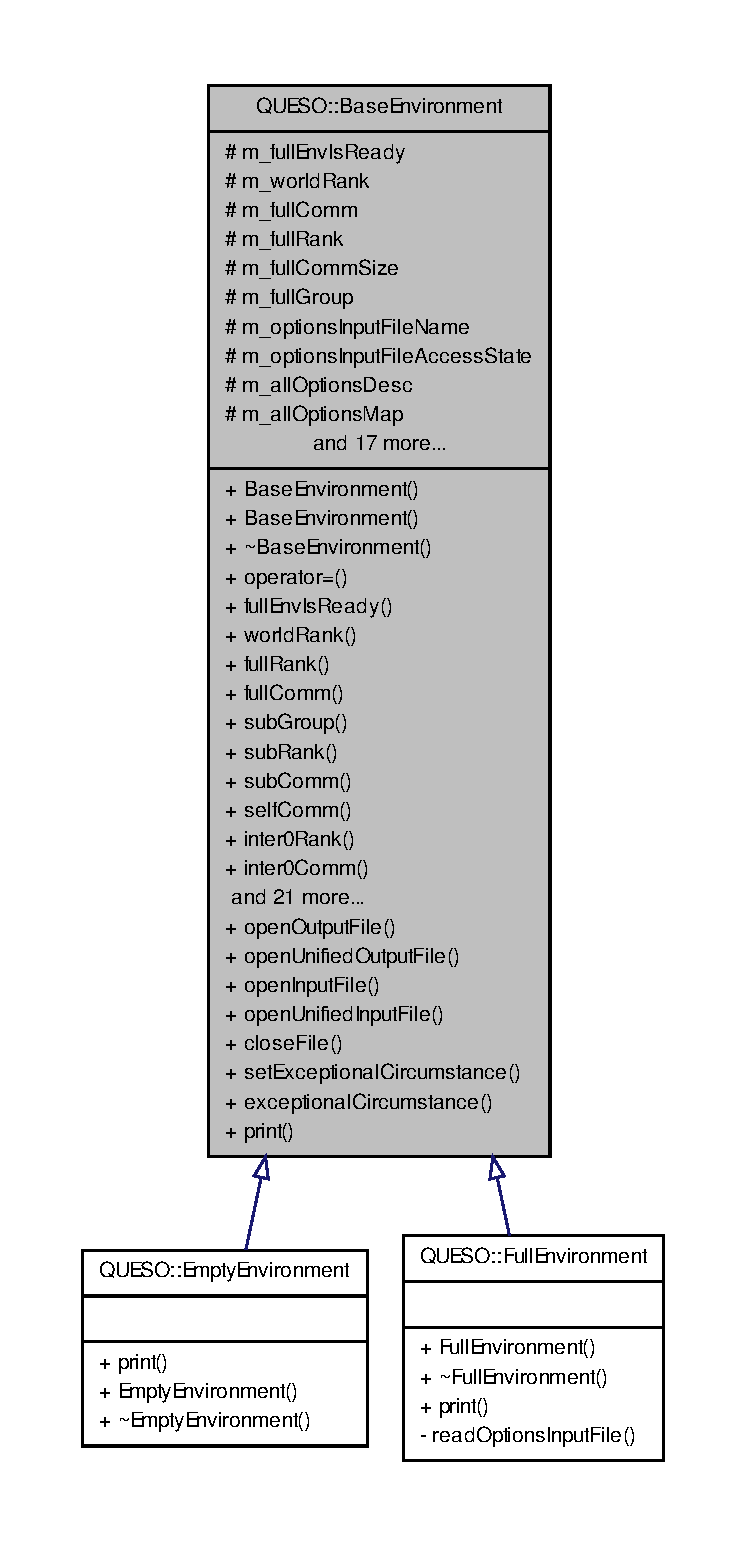
\includegraphics[scale=0.80,clip=true]{rawfigs/base_env_class.pdf}
\vspace*{-1.2cm}
\caption{The class diagram for the {Environment} class described in Section \ref{sec:environment_class}.}
\label{fig-env-class}
\end{figure}

\begin{figure}[!hp]
\centering
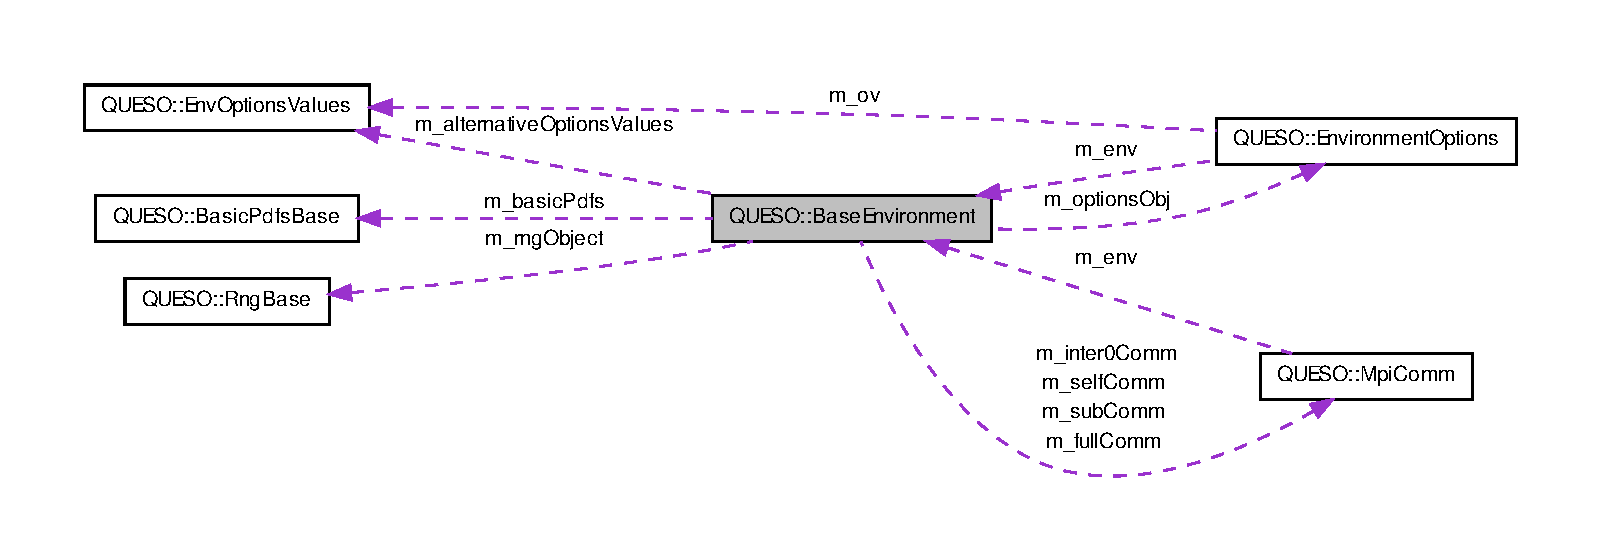
\includegraphics[scale=0.60,clip=true]{rawfigs/base_env_coll.pdf}
\vspace*{-1.cm}
\caption{Collaboration graph for the environment class described in Section \ref{sec:environment_class}.}
\label{fig-env-coll}
\end{figure}

\begin{figure}[htpb]
\centering
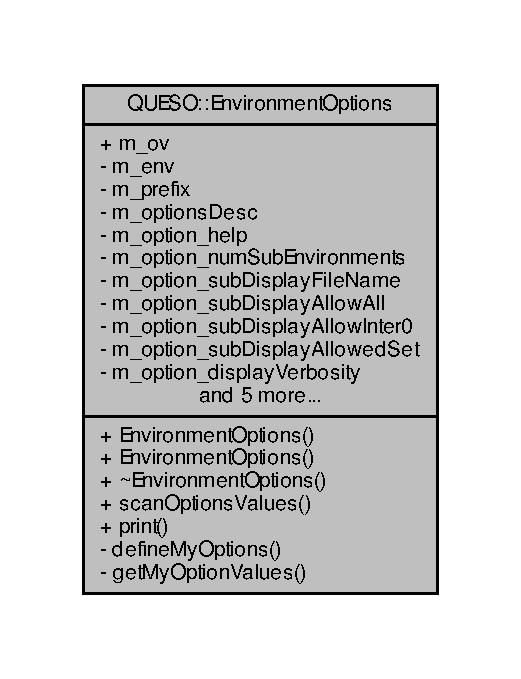
\includegraphics[scale=0.8,clip=true]{rawfigs/environment_options}
\vspace*{-1.2cm}
\caption{The environment options class with its attributes and methods.}
\label{fig-env-options-class}
\end{figure}

% \begin{figure}[!hp]
% \centering
% \includegraphics[scale=0.60,clip=true]{rawfigs/class_q_u_e_s_o_1_1_environment_options__coll__graph.pdf}
% \vspace*{-1.2cm}
% \caption{Collaboration graph for the environmentOption class.}% described in Section \ref{sec:environment_class}.}
% \label{fig-env-options-col}
% \end{figure}


% 
%\subsubsection{Input File Options}


\begin{table}[htpb]
\begin{center}
\caption{Input file options for a QUESO environment.}
\vspace{-8pt}
\label{tab-env-options}
\footnotesize
\begin{tabular}{l c  m{7cm}}
\toprule
Option name                      &  Default  value & Description \\
\midrule\midrule
\ttfamily \textlangle PREFIX\textrangle env\_help                &     & Produces help message for environment class            \\
%\midrule
\ttfamily\textlangle PREFIX\textrangle env\_numSubEnvironments   &  1  &  Number of subenvironments                \\ %UQ_ENV_NUM_SUB_ENVIRONMENTS_ODV
% \midrule
\ttfamily\textlangle PREFIX\textrangle env\_subDisplayFileName   & \ttfamily"." & Output filename for sub-screen writing     \\ %UQ_ENV_SUB_DISPLAY_FILE_NAME_ODV
% \midrule
\ttfamily\textlangle PREFIX\textrangle env\_subDisplayAllowAll   &  0  & Allows all subenvironments to write to output file \\ %UQ_ENV_SUB_DISPLAY_ALLOW_ALL_ODV
% \midrule
\ttfamily\textlangle PREFIX\textrangle env\_subDisplayAllowedSet & \ttfamily""  & Subenvironments that will write to output file \\ %UQ_ENV_SUB_DISPLAY_ALLOWED_SET_ODV
% \midrule
\ttfamily\textlangle PREFIX\textrangle env\_displayVerbosity     &  0  & Sets verbosity				         \\ %UQ_ENV_DISPLAY_VERBOSITY_ODV
% \midrule
\ttfamily\textlangle PREFIX\textrangle env\_syncVerbosity        &  0  & Sets syncronized verbosity             \\ %UQ_ENV_SYNC_VERBOSITY_ODV
% \midrule
\ttfamily\textlangle PREFIX\textrangle env\_seed                 &  0  & Set seed                             \\ %UQ_ENV_SEED_ODV
%
% TODO add the following options:
% (m_option_platformName.c_str(),         po::value<std::string >()->default_value(UQ_ENV_PLATFORM_NAME_ODV),           "platform name")""
% (m_option_identifyingString.c_str(),    po::value<std::string >()->default_value(UQ_ENV_IDENTIFYING_STRING_ODV),      "identifying string")""
% (m_option_checkingLevel.c_str(),        po::value<unsigned int>()->default_value(UQ_ENV_CHECKING_LEVEL_ODV),          "set checking level")  0          
\bottomrule
\end{tabular}
\end{center}
\end{table}

  

%\clearpage
\subsection{Vector}\label{sec:vector_class}


The Vector class handles all the vector operations carried out in QUESO, and currently has two derived classes: \verb+GslVector+ and \verb+TeuchosVector+. \verb+GslVector+ is based on the GSL vector structure; whereas \verb+TeuchosVector+ is based on Trilinos Teuchos vector structure~\cite{Trilinos}, and therefore, it is only available if QUESO was compiled with Trilinos.  

A class diagram for \verb+Vector+ class is presented in Figure \ref{fig-vector-class}.%; the reader may notice that the diagram also presents an extra class, \verb+PetscVector+, in order to show QUESO flexibility to the inclusion of other classes -- this class has yet to be implemented.


\begin{figure}[!htpb]
\centering
\vspace*{-.5cm}
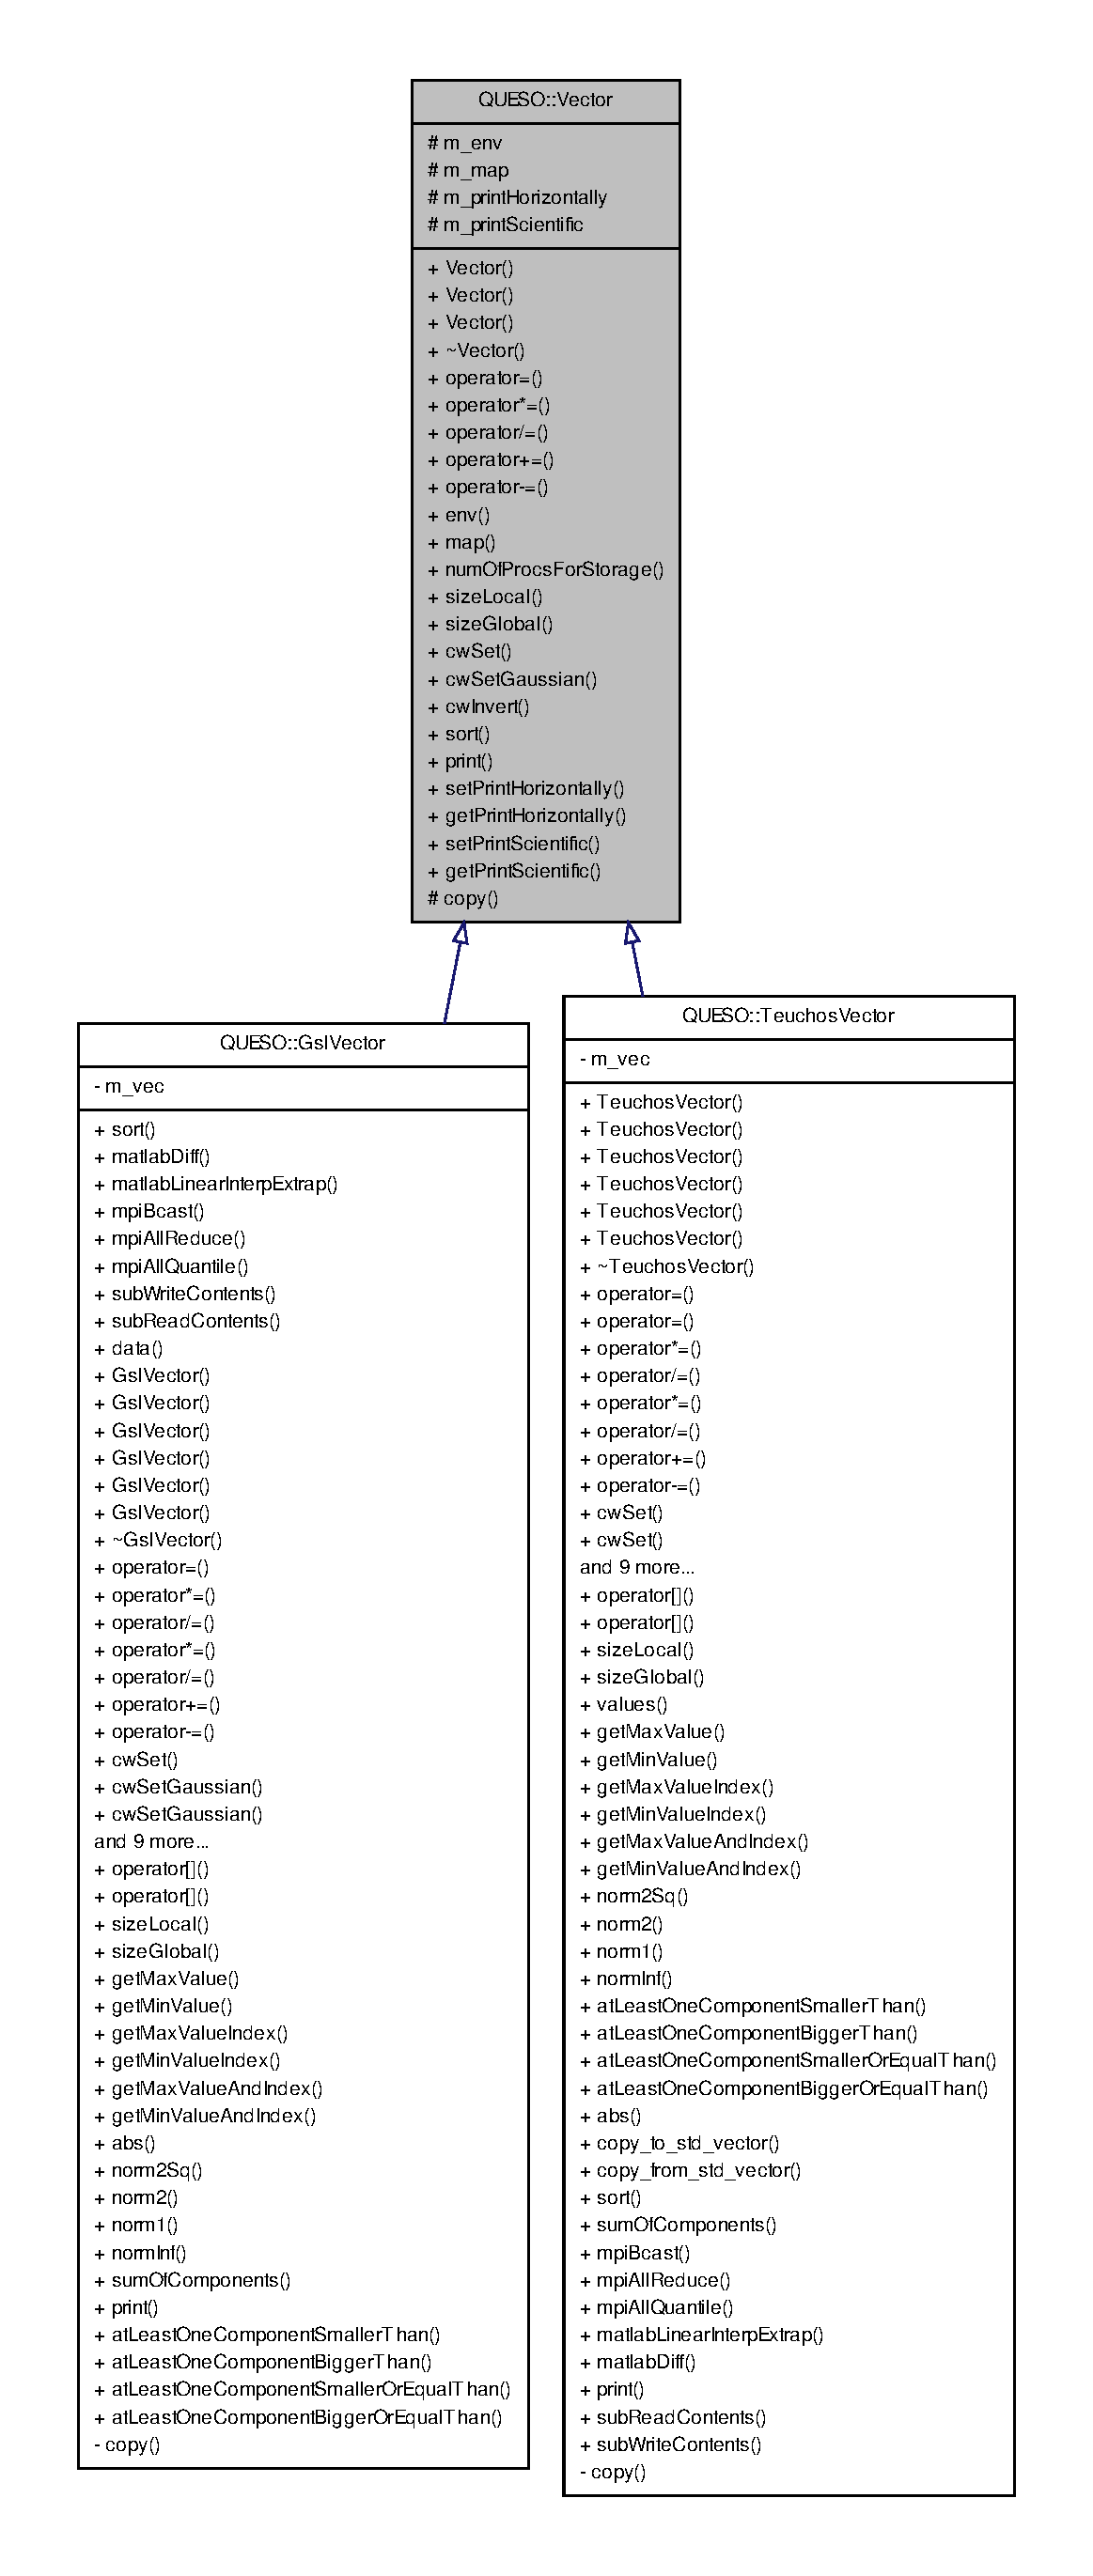
\includegraphics[scale=0.50,clip=true]{rawfigs/vector}
\vspace*{-.8cm}
\caption{ The class diagram for the vector class described in Section \ref{sec:vector_class}.}
\label{fig-vector-class}
\end{figure}



\subsection{Matrix}\label{sec:matrix_class}

% The Matrix class handles all the matrix operations carried out in QUESO, and its class diagram is presented in Figure \ref{fig-matrix-class}. Analogously to the Vector class case,
% Matrix class has two derived classes: \verb+GslMatrix+ and \verb+TeuchosMatrix+. \verb+GslMatrix+ is based on the GSL matrix structure; whereas \verb+TeuchosMatrix+ is based on Trilinos Epetra matrix structure.


The Matrix class handles all the matrix operations carried out in QUESO.  Analogously to the vector class case described in the previous section,
matrix class currently has two derived classes: \verb+GslMatrix+ and \verb+TeuchosMatrix+. \verb+GslMatrix+ is based on the GSL matrix structure; whereas \verb+TeuchosMatrix+ is based on Trilinos Epetra matrix structure.

A class diagram for \verb+Matrix+  is presented in Figure \ref{fig-matrix-class}; it displays its protected attributes together with its member functions. Again, the diagram displays in some detail the inherited classes \verb+GslMatrix+ and \verb+TeuchosMatrix+.


\begin{figure}[!hp]
\centering
\vspace*{-.8cm}
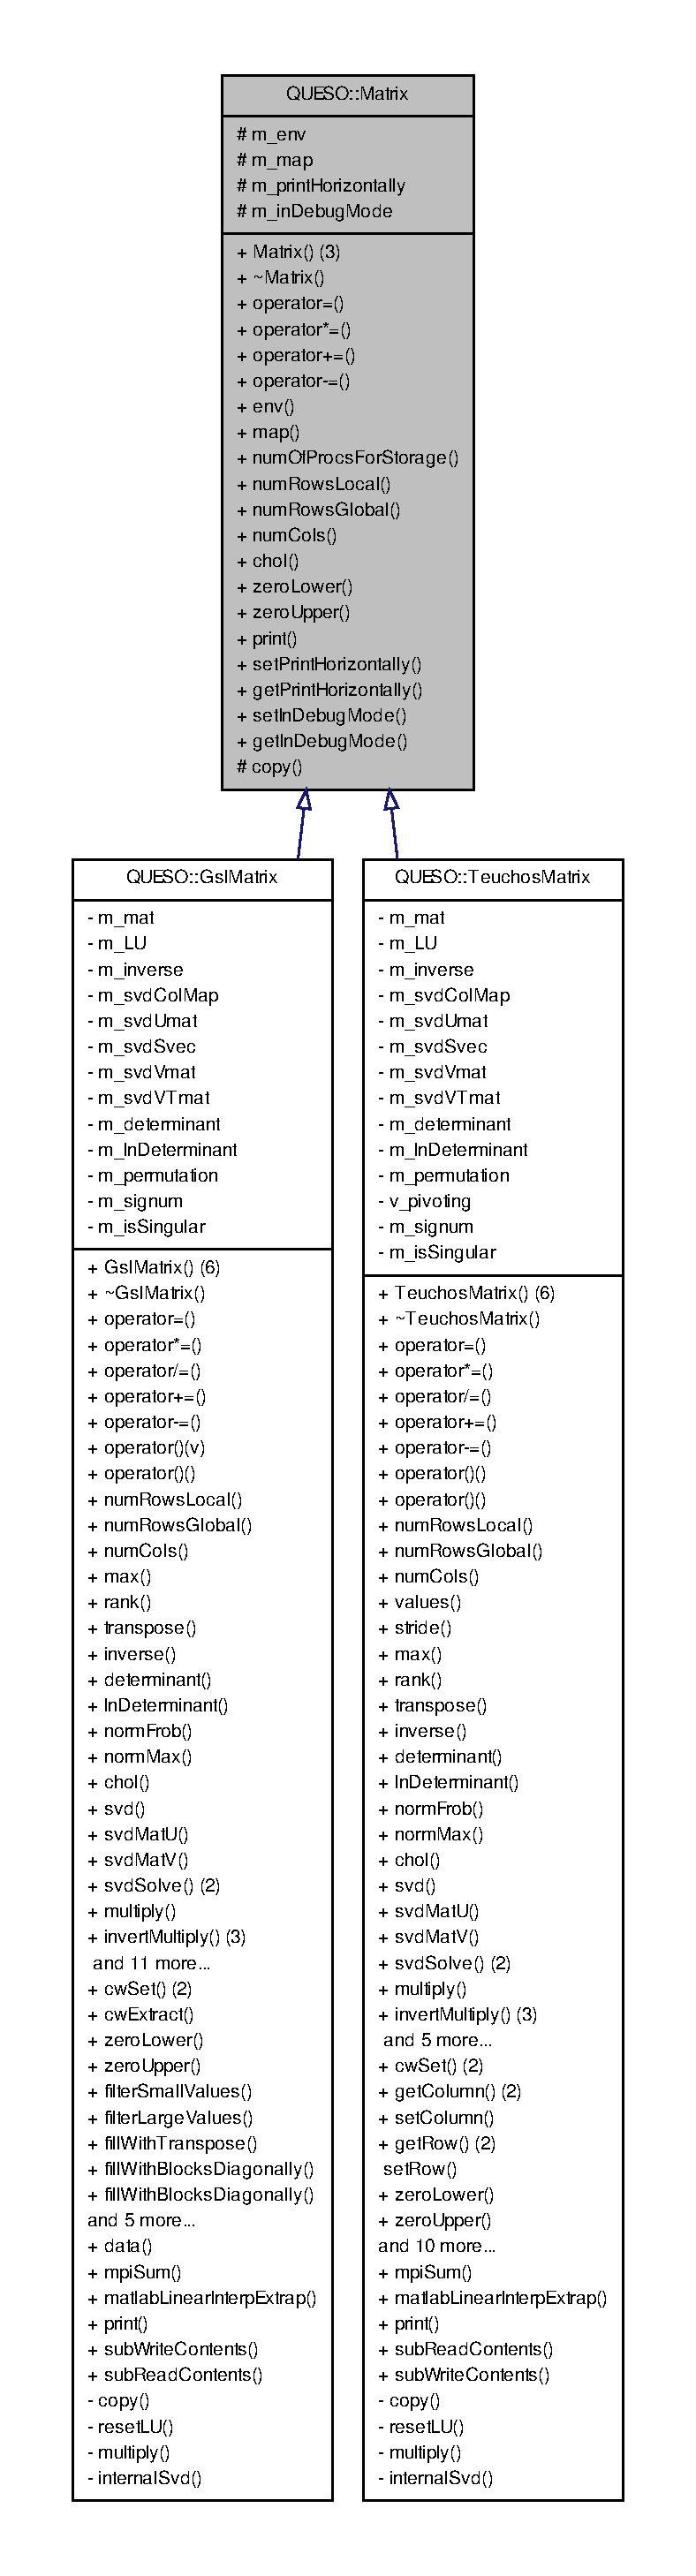
\includegraphics[scale=0.50,clip=true]{rawfigs/matrix}
\vspace*{-.8cm}
\caption{The class diagram for the matrix class.}% described in Section \ref{sec:matrix_class}.}
\label{fig-matrix-class}
\end{figure}


%\clearpage
\section{Templated Basic Classes}
The classes in this group are: vector sets, subsets and spaces (Section \ref{sec:vector-set-space}), scalar and vector function classes (Section \ref{sec:scalar-vector-function}), and scalar and vector sequences (Section \ref{sec:scalar-vector-sequence}).

These classes constitute the core entities necessary for the formal
mathematical definition and description of other entities, such as
random variables, Bayesian solutions of inverse problems, sampling algorithms and chains.

%\clearpage


\subsection{Vector Set, Subset  and Vector Space Classes}\label{sec:vector-set-space}
%
The vector set class is fundamental for the proper handling of many mathematical entities.
Indeed, the definition of a scalar function such as $\pi:\mathbf{B}\subset\mathbb{R}^n\rightarrow\mathbb{R}$ requires the
specification of the domain $\mathbf{B}$, which is a {\it subset} of the {\it vector space} $\mathbb{R}^n$, which is itself a {\it set}. Additionally, 
 SIPs need a likelihood routine $\pi_{\text{like}}:\mathbb{R}^n\rightarrow\mathbb{R}_+$,
and SFPs need a QoI routine $\mathbf{q}:\mathbb{R}^n\rightarrow\mathbb{R}^m$; the \textit{sets} $\mathbb{R}^n$, $\mathbb{R}^m$, etc., are {\it vector spaces}.


The relationship amongst QUESO classes for handling sets, namely \verb+VectorSet+; subsets, namely \verb+VectorSubset+;  and vector spaces, namely \verb+VectorSpace+ is sketched in Figure \ref{fig-vector-space-subset-classes}.
%
An attribute of the {\it subset} class is the {\it vector space} which it belongs to, and in fact a reference to a vector space is required by the constructor of the subset class. An example of this case is the definition of a scalar function such as $\pi:\mathbf{B}\subset\mathbb{R}^n\rightarrow\mathbb{R}$ above. %, which requires the specification of the domain $\mathbf{B}$, which is a {\it subset} of the {\it vector space} $\mathbb{R}^n$, which is itself a {\it set}.

The power of an object-oriented design is clearly featured here.
The intersection subset derived class \verb+IntersectionSubset+ is useful for handling a posterior PDF  on Equation~\eqref{eq-Bayes-solution},
since its domain is the intersection of the domain of the prior PDF with the domain of the likelihood function.

\begin{figure}[htpb]
% \centering
\hspace{-1cm}
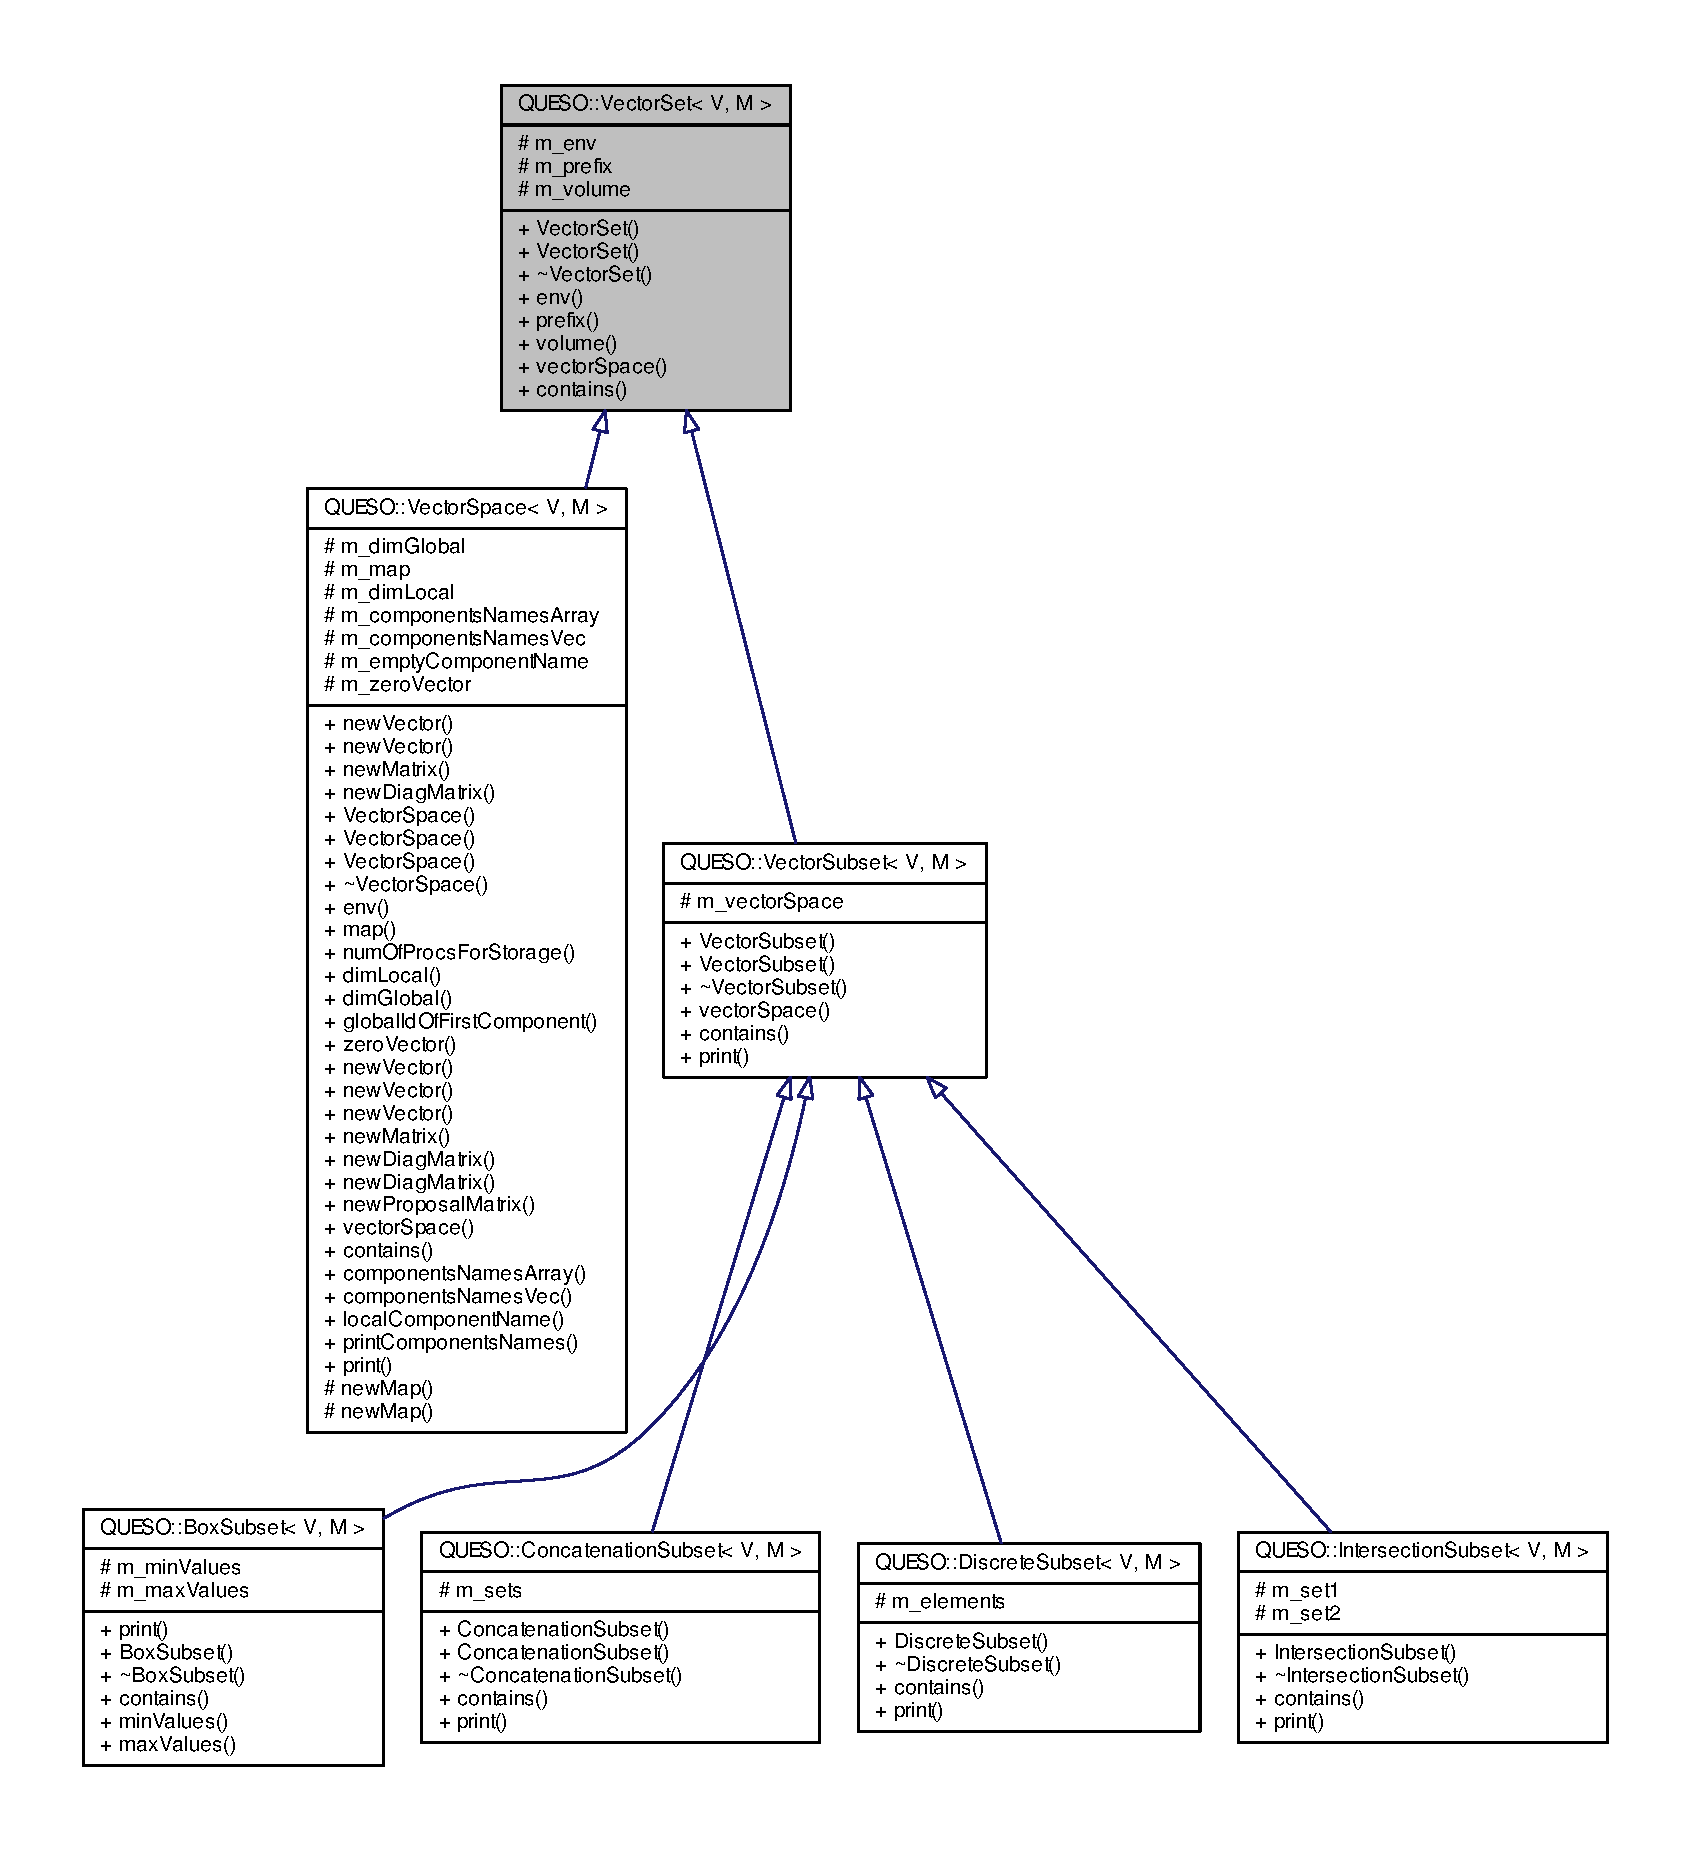
\includegraphics[scale=0.65,clip=true]{rawfigs/vector_set}
\vspace*{-1.5cm}
\caption{The class diagram for vector set, vector subset and vector space classes, described in Section \ref{sec:vector-set-space}.}
\label{fig-vector-space-subset-classes}
\end{figure}

% 
% \begin{figure}[htpb]
% % \centering
% \hspace{-1cm}
% \includegraphics[scale=0.65,clip=true]{rawfigs/class_q_u_e_s_o_1_1_vector_set__coll__graph}
% \vspace*{-1.5cm}
% \caption{Collaboration graph of VectorSet class.}
% \label{fig-vector-space-subset-classes}
% \end{figure}



%\clearpage
\subsection{Scalar Function and Vector Function Classes}\label{sec:scalar-vector-function}

Joint PDF, marginal PDF, and CDF are all examples of scalar functions present in statistical problems. 
QUESO currently supports basic PDFs such as uniform and Gaussian and also more complex PDFs, such as the ones coming from a Bayesian analysis. They are implemented in the classes \verb+UniformJointPdf+, \verb+GaussianJointPdf+, and \verb+BayesianJointPdf+, respectively. The posterior PDF may be represented within QUESO by \verb+GenericJointPdf+.
See Diagram~\ref{fig-scalar-function-class} for the scalar function class.

The handling of vector functions within QUESO is also quite straightforward. Indeed, the definition of a vector function $\mathbf{q}:\mathbf{B}\subset\mathbb{R}^n\rightarrow\mathbb{R}^m$ requires only the extra specification of the image vector space $\mathbb{R}^m$. The classes representing the vector function class \verb+GenericVectorFunction+ and \verb+ConstantVectorFunction+ are derived  from \verb+BaseVectorFunction+ and are presented in Diagram \ref{fig-vector-function-class} 
\begin{figure}[htpb]
% \centering
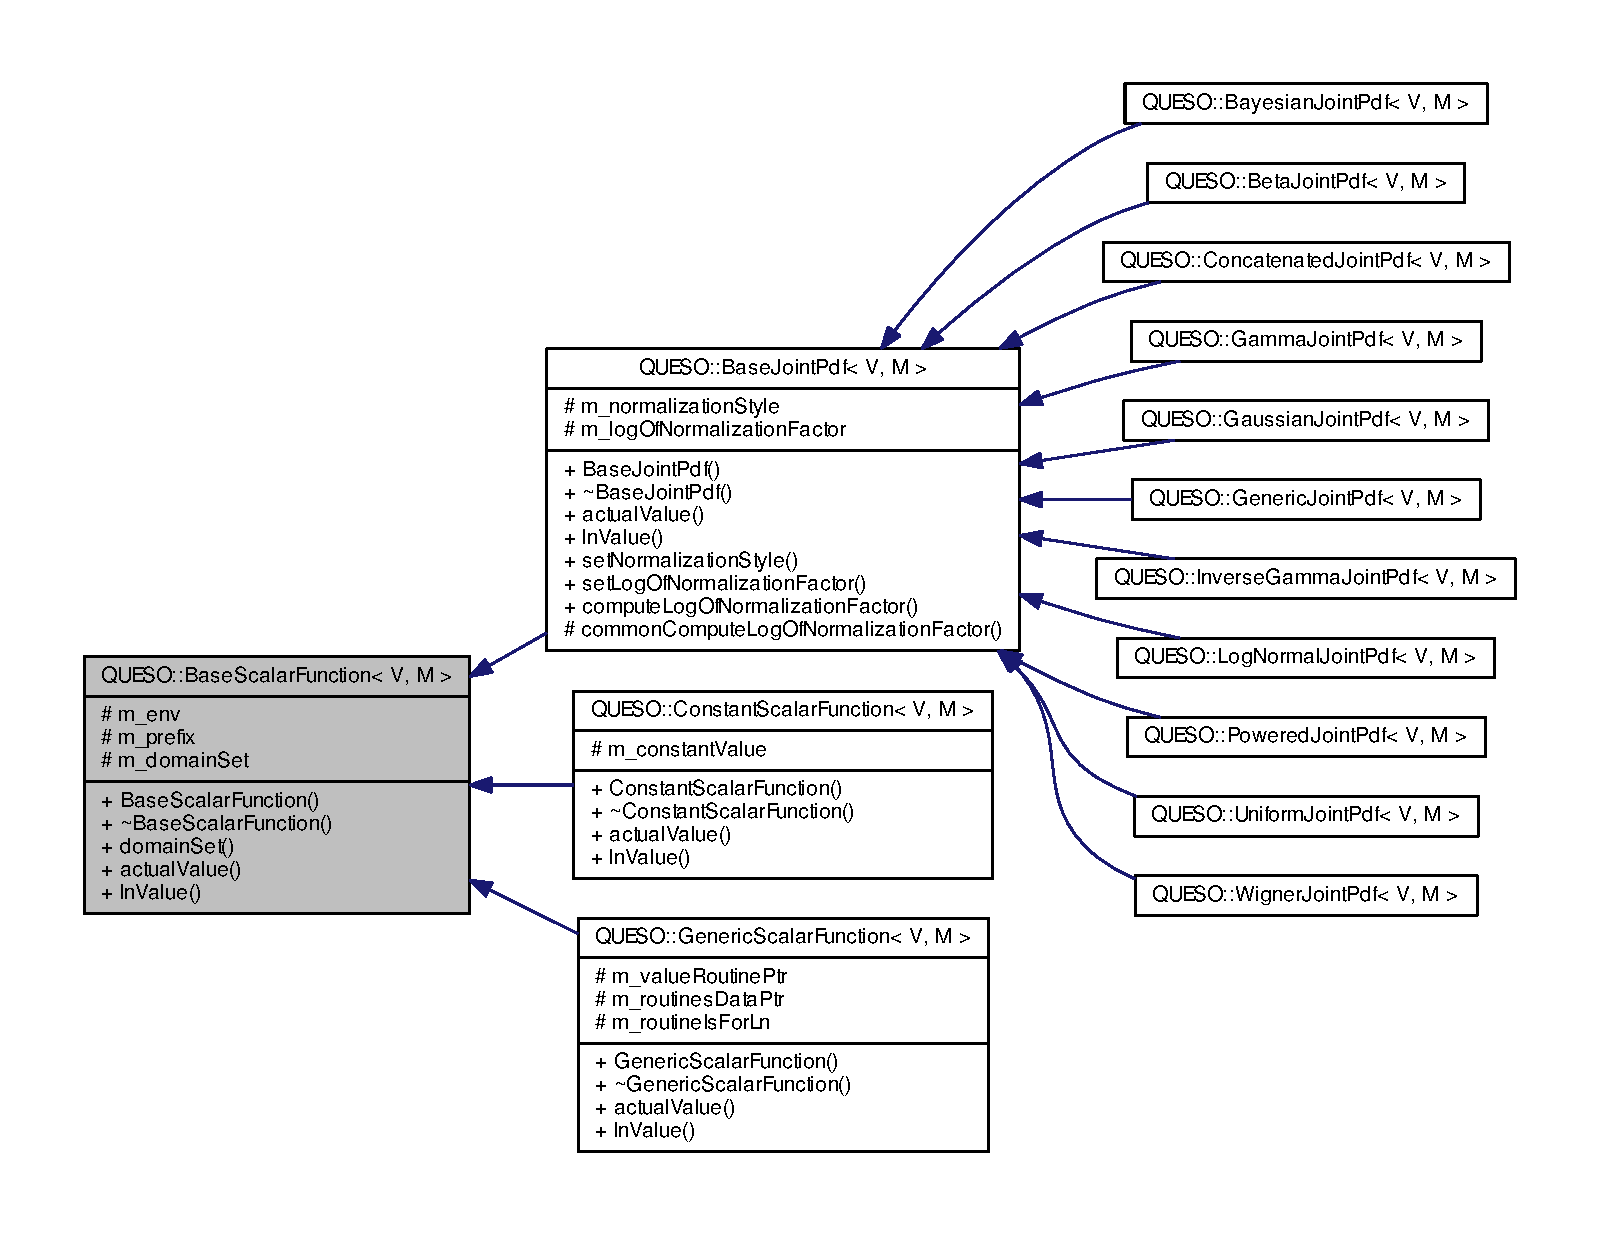
\includegraphics[scale=0.65,clip=true]{rawfigs/base_scalar_function}
\vspace*{-1.5cm}
\caption{The class diagram for the scalar function class.}
\label{fig-scalar-function-class}
\end{figure}

\begin{figure}[htpb]
\centering
\hspace{-40pt}
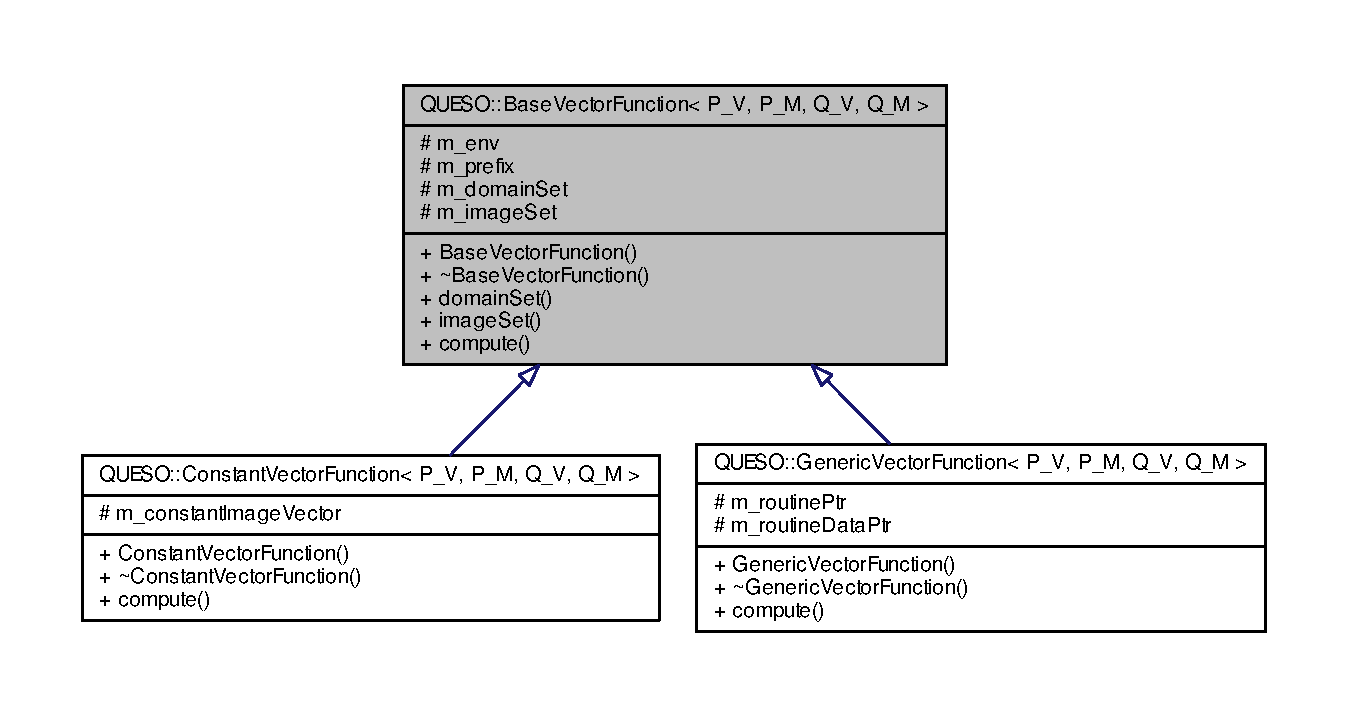
\includegraphics[scale=0.65,clip=true]{rawfigs/base_vector_function.pdf}
\vspace{-1.2cm}
\caption{The class diagram for the vector function class described in Section \ref{sec:scalar-vector-function}.} % new fig: added uqConstantVectorFunctionClass on 12/17/12.
\label{fig-vector-function-class}
\end{figure}

%\clearpage

\subsection{Scalar Sequence and Vector Sequence Classes}\label{sec:scalar-vector-sequence}
%
The scalar sequence class contemplates {\it scalar} samples generated by an algorithm, as well as operations that can
be done over them, e.g., calculation of means, variances, and convergence indices.
%% such as Geweke and Brooks-Gelman.
Similarly, the vector sequence class contemplates {\it vector} samples and operations such as means, correlation matrices and covariance matrices.

Figures \ref{fig-scalar-sequence-class} and \ref{fig-vector-sequence-class} display the class diagram for the scalar sequence  and vector sequence classes, respectively.

\begin{figure}[htpb]
\centering
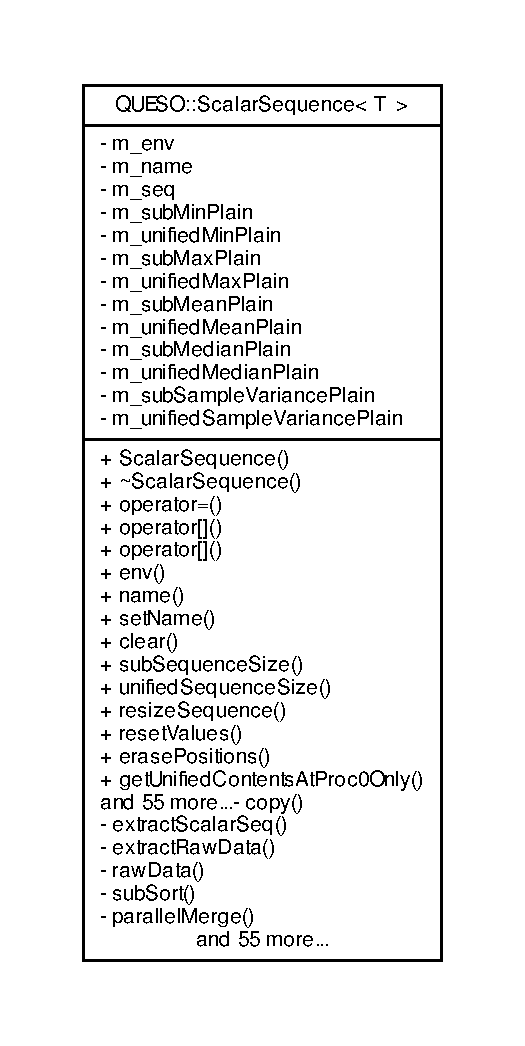
\includegraphics[scale=0.65,clip=true]{rawfigs/scalar_sequence}
\vspace{-1.cm}
\caption{The class diagram for the scalar sequence class.}
\label{fig-scalar-sequence-class}
\end{figure}

\begin{figure}[htpb]
\centering
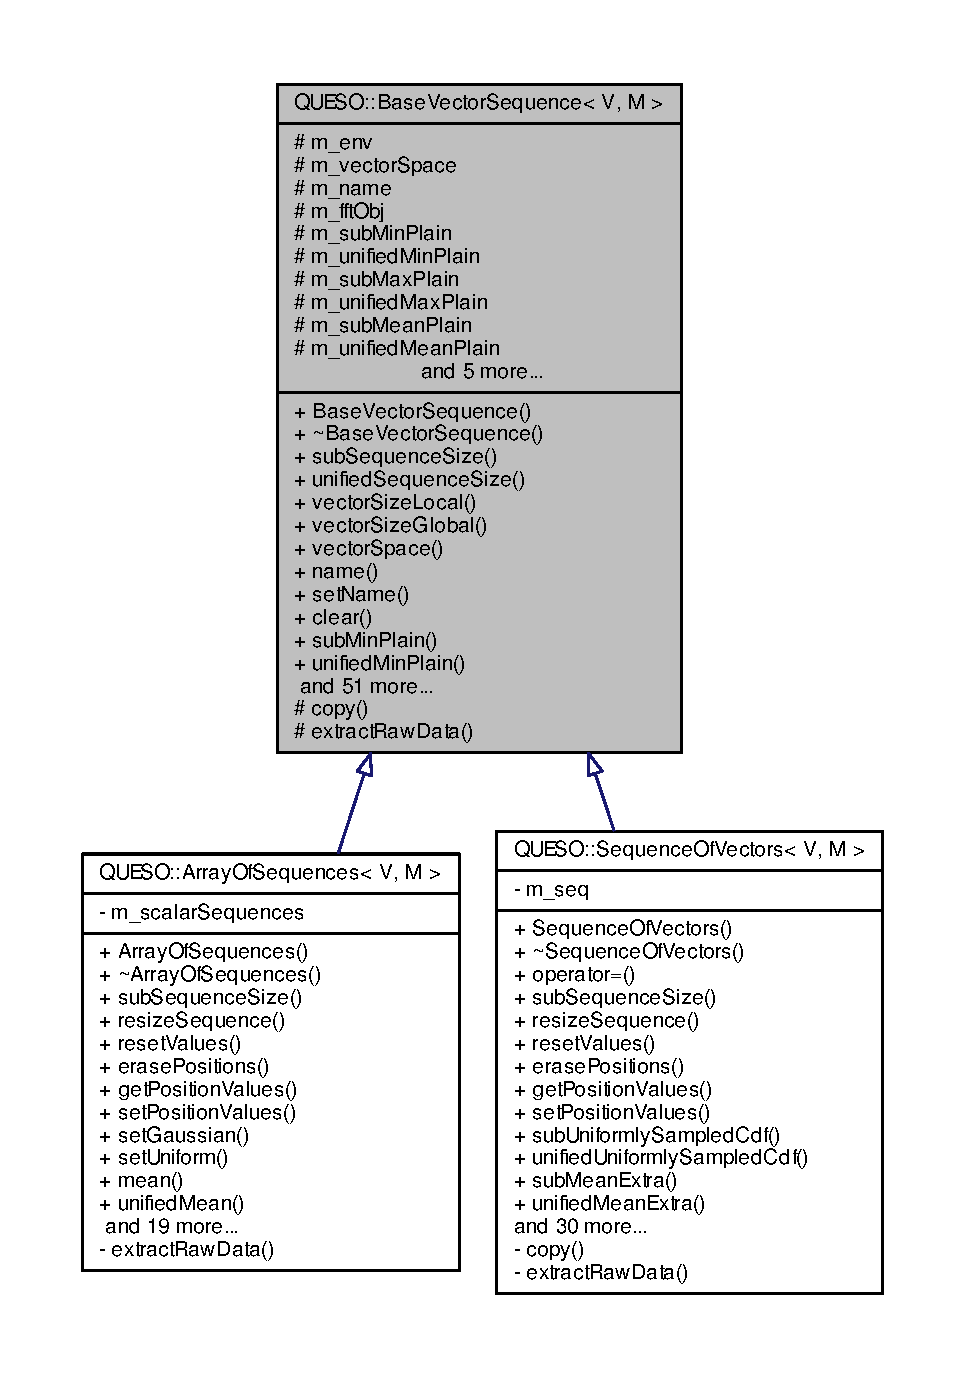
\includegraphics[scale=0.65,clip=true]{rawfigs/vector_sequence}
\vspace{-1.cm}
\caption{The class diagram for the vector sequence class.}
\label{fig-vector-sequence-class}
\end{figure}



%\clearpage
\section{Templated Statistical Classes}

The classes in this group are: vector realizer, vector random variable, statistical inverse problem (and options), Metropolis-Hastings solver (and options), statistical forward problem (and options), Monte Carlo solver (and options), and Sequence statistical options.

For QUESO, a SIP has two input entities, a prior RV and
a likelihood routine, and one output entity, the posterior RV, as shown in Chapter \ref{ch-introduction}, Figure~\ref{fig-sip-queso}.
%
Similarly, a SFP has two input entities, a input RV and
a QoI routine, and one output entity, the output RV, as shown in Figure \ref{fig-sfp-queso}.


\subsection{Vector Realizer Class}\label{sec:vector-realizer-class}
%
A {\it realizer} is an object that, simply put, contains a \verb+realization()+ operation that returns a sample of a vector RV.
QUESO currently supports several realizers: 
\begin{itemize}
 \item uniform, implemented in \verb+UniformVectorRealizer+,                \vspace{-8pt}
\item Gaussian, implemented in \verb+GaussianVectorRealizer+,               \vspace{-8pt}
\item Log Normal, implemented in \verb+LogNormalVectorRealizer+,            \vspace{-8pt}
\item Gamma,  implemented in \verb+GammaVectorRealizer+,                    \vspace{-8pt}
\item Inverse Gamma, implemented in \verb+InverseGammaVectorRealizer+, and  \vspace{-8pt}
\item Beta, , implemented in \verb+BetaVectorRealizer+,                     \vspace{-8pt}
\end{itemize}
which are all derived from the base class \verb+BaseVectorRealizer+. 
 
QUESO conveniently provides the class \verb+ConcatenatedVectorRealizer+, which allows two distinct realizers to be concatenated.
It also contains a {\it sequence realizer} class for storing samples of a MH algorithm. 




\subsection{Vector Random Variable Class}
%
Vector RVs are expected to have two basic functionalities:
compute the value of its PDF at a point, and generate realizations following such PDF.
The joint PDF (\verb+BaseJointPdf+ and derived classes, see Section \ref{sec:scalar-vector-function}) and vector realizer  (\verb+BaseVectorRealizer+ and derived classes, see Section \ref{sec:vector-realizer-class}) classes allow a straightforward definition and manipulation of vector RVs. Similarly to the vector realizer class above, QUESO also allows users to form new RVs through the concatenation of existing RVs (class \verb+ConcatenatedVectorRV+).

QUESO currently supports a few vector RVs such as uniform, Gaussian, Gamma and Beta, as depicted in Diagram \ref{fig-vector-rv-class}.
A derived class called {\it generic vector RV} allows QUESO to store the solution of an statistical IP:
a {\it Bayesian joint PDF} becomes the PDF of the posterior RV, while a {\it sequence vector realizer} becomes the realizer of the same posterior RV.



\begin{figure}[htpb]
\centering
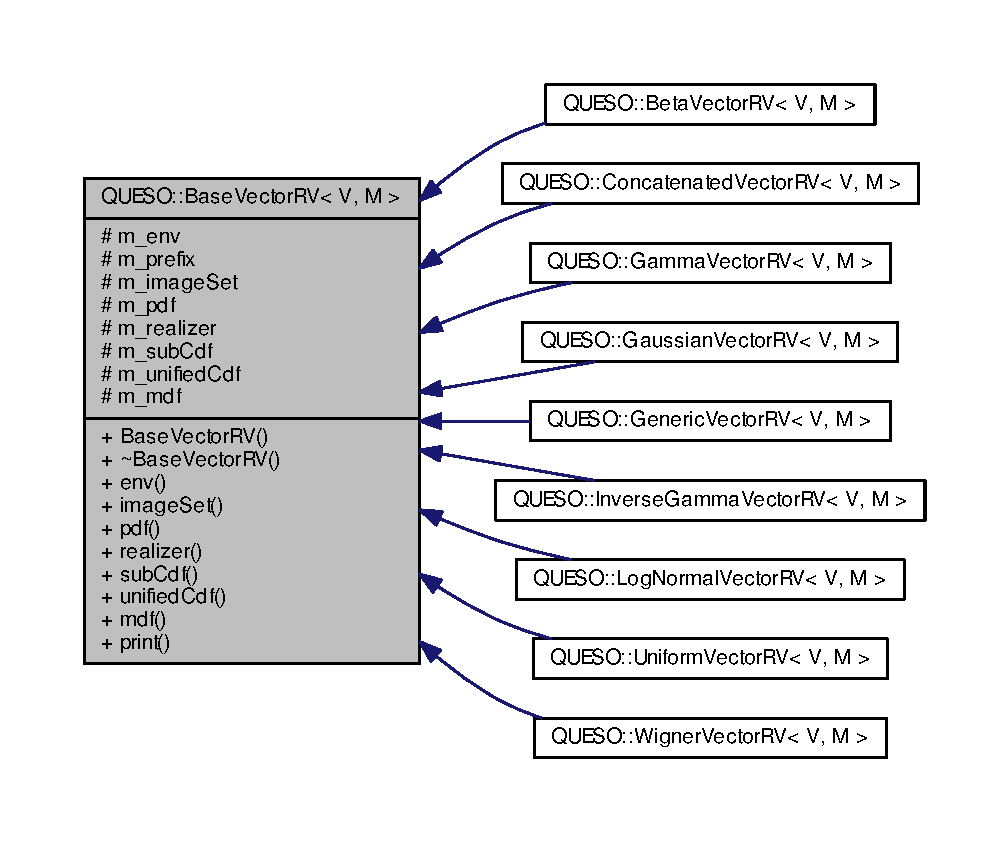
\includegraphics[scale=0.7,clip=true]{rawfigs/vector_rv}
\vspace{-1.cm}
\caption{The class diagram for the vector random variable class.}
\label{fig-vector-rv-class}
\end{figure}



%\clearpage
\subsection{Statistical Inverse Problem (and Options)}
Similarly to its mathematical concepts, a SIP in QUESO also expects two input entities, a prior RV and a likelihood routine, and one output entity, the posterior RV.
The SIP is represented in QUESO through the templated class \verb+StatisticalInverseProblem<P_V,P_M>+, which is illustrated in Figure \ref{fig-sip-class}.
One important characteristic of the QUESO design is that it  separates `what the problem is' from `how the problem is solved'.
The prior and the posterior RV are instances of the \verb+BaseVectorRv<V,M>+ class, while
the likelihood function is an instance of the \verb+BaseScalarFunction<V,M>+ class.

The solution of a SIP is computed by calling either \verb+solveWithBayesMetropolisHastings()+ or \verb+solveWithBayesMLSampling()+, which are member functions of the class\linebreak\verb+StatisticalInverseProblem<P_V,P_M>+ class.
Upon return from a solution operation, the posterior RV is available through the \verb+postRv()+ member function.
More details are provided about \verb+solveWithBayesMetropolisHastings()+ and \verb+solveWithBayesMLSampling()+ in Sections \ref{sec:MH} and \ref{sec:ML}, respectively.

Figure \ref{fig-sip-options-class} displays the  \verb+StatisticalInverseProblemOptions+ class, i.e. that class that handles a variety of options for solving the SIP. Such options may be provided to QUESO by the user's input file; and they are listed in Table \ref{tab-sip-options}.


\begin{figure}[htpb]
\centering
\subfloat[StatisticalInverseProblem]{
 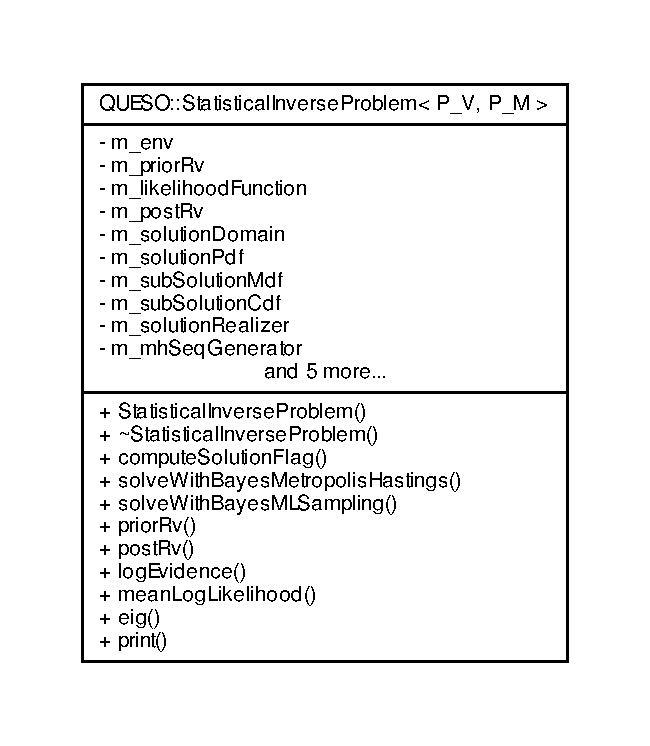
\includegraphics[trim={0 1.3cm 0 0},clip,scale=0.8]{rawfigs/statistical_inverse_problem}\label{fig-sip-class}}
\subfloat[StatisticalInverseProblemOptions]{
 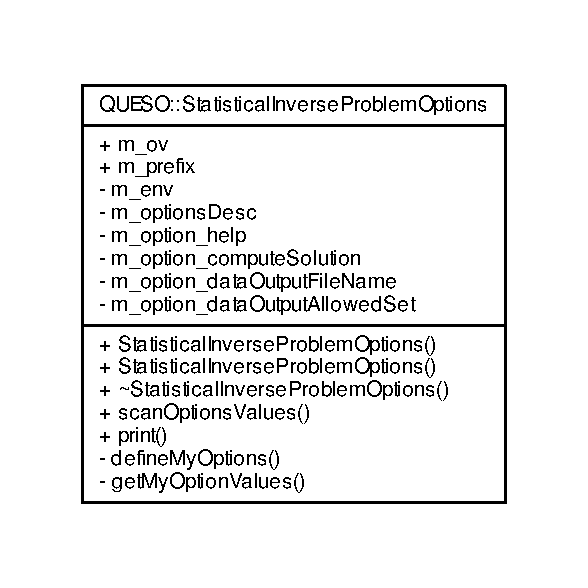
\includegraphics[trim={0 1.3cm 0 0},clip,scale=0.8]{rawfigs/statistical_inverse_problem_options}\label{fig-sip-options-class}}
\vspace{-.2cm}
\caption{The statistical inverse problem class, which implements the representation in Figure~\ref{fig-sip-queso}, and statistical inverse problem options class.}
\end{figure}



\begin{table}[htpb]
\begin{center}
\caption{Input file options for a QUESO statistical inverse problem.}
\vspace{-8pt}
\label{tab-sip-options}
\ttfamily\footnotesize
\begin{tabular}{l c  m{7cm}}
\toprule
\rmfamily Option name                    & \rmfamily Default  Value & \rmfamily Description \\
\midrule\midrule
\textlangle PREFIX\textrangle ip\_help                 &     &  \rmfamily Produces help message for statistical inverse problem   \\
% \midrule
\textlangle PREFIX\textrangle ip\_computeSolution      &  1  &  \rmfamily Computes solution process \\% UQ_SIP_COMPUTE_SOLUTION_ODV
% \midrule
\textlangle PREFIX\textrangle ip\_dataOutputFileName   & "." &  \rmfamily Name of data output file \\%UQ_SIP_DATA_OUTPUT_FILE_NAME_ODV
% \midrule
\textlangle PREFIX\textrangle ip\_dataOutputAllowedSet & ""  &  \rmfamily Subenvironments that will write to data output file  \\%UQ_SIP_DATA_OUTPUT_ALLOWED_SET_ODV
\bottomrule
\end{tabular}
\end{center}
\end{table}


%\clearpage
\subsection{Metropolis-Hastings Solver (and Options)}\label{sec:MH}


The templated class that represents a Metropolis-Hastings generator of samples in QUESO is \verb+MetropolisHastingsSG<P_V,P_M>+, where SG stands for 'Sequence Generator'. This class implements the DRAM algorithm of Haario, Laine, Mira and Saksman~\cite{HaLaMiSa06} together with an operation named \verb+generateSequence()+ 
based on the core routine at the MCMC toolbox for MATLAB~\cite{Mcmctool}. %In fact,, the reader may notice that the example available in the QUESO build tree directory \verb+examples/statisticalInverseProblem+ is closely related to the `normal example' in the toolbox.


The Metropolis-Hastings sequence generator class is depicted in Figure \ref{fig-metropolis-hastings-solver-class}; the Metropolis-Hastings sequence generator options class is depicted in Figure \ref{fig-metropolis-hastings-options-class}. A collaboration graph for the Metropolis-Hastings class is presented in Figure \ref{fig-metropolis-hastings-coll}; and the options are presented in Table \ref{tab-metropolis-hastings-options}.

% \begin{figure}[htpb]
% \centering
% \subfloat[MetropolisHastingsSG]{\label{fig-metropolis-hastings-solver-class}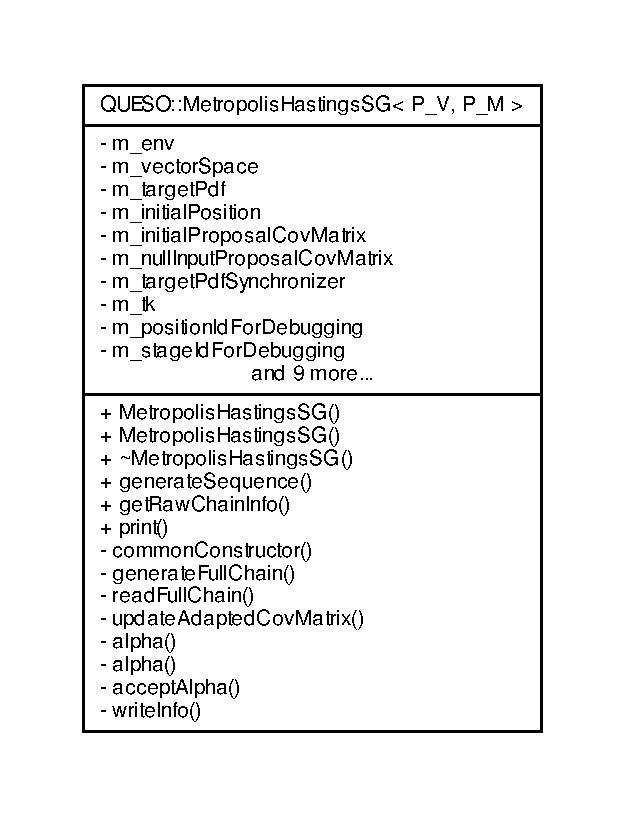
\includegraphics[trim={0 1.3cm 0 0},clip, scale=0.65]{rawfigs/metropolis_hastings}}
% \subfloat[MetropolisHastingsSGOptions]{\label{fig-metropolis-hastings-options-class}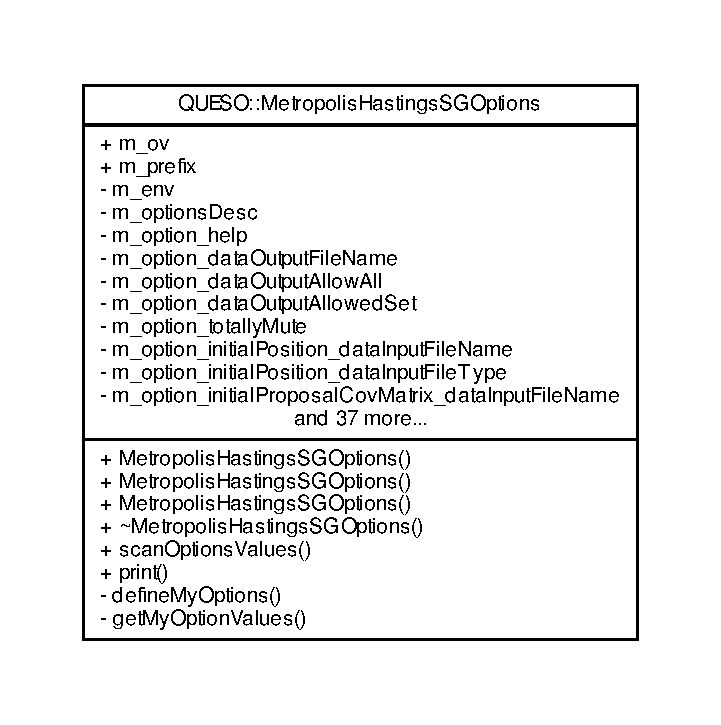
\includegraphics[trim={0 1.3cm 0 0},clip, scale=0.65]{rawfigs/metropolis_hastings_options}}
% \vspace{-.2cm}
% \caption{The Metropolis-Hastings sequence generator class and the Metropolis-Hastings sequence generator options class.}
% \end{figure}


\begin{figure}[htpb]
\centering
\subfloat[MetropolisHastingsSG]{\label{fig-metropolis-hastings-solver-class}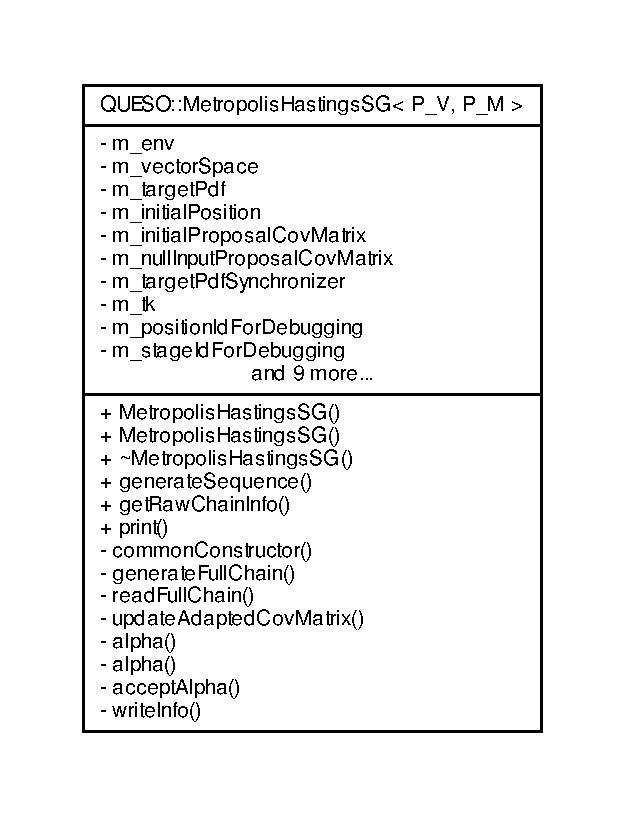
\includegraphics[trim={0 1.3cm 0 0},clip, scale=0.65]{rawfigs/metropolis_hastings}}
\subfloat[MetropolisHastingsSGOptions]{\label{fig-metropolis-hastings-options-class}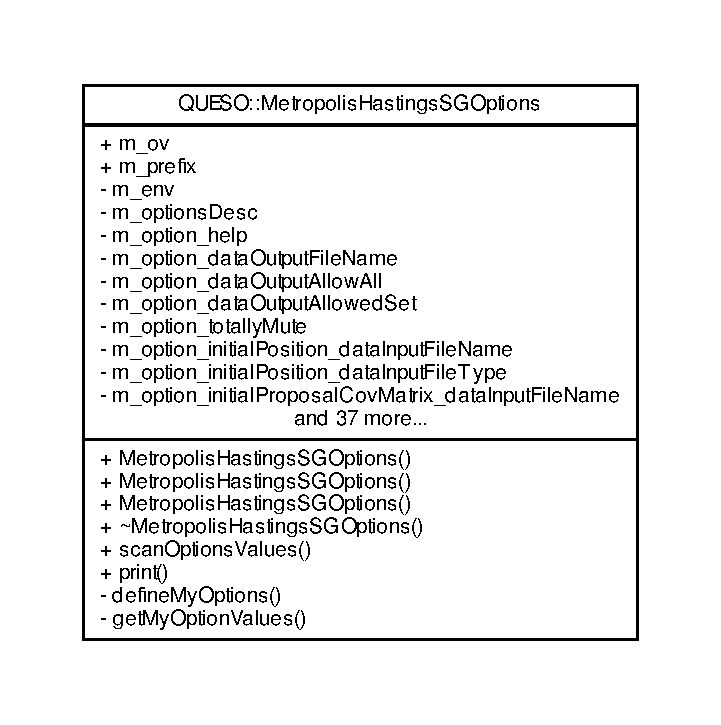
\includegraphics[trim={0 1.3cm 0 0},clip, scale=0.65]{rawfigs/metropolis_hastings_options}}
\vspace{-.2cm}
\caption{The Metropolis-Hastings sequence generator class and the Metropolis-Hastings sequence generator options class.}
\end{figure}

% Use the trim option, which takes four space separated values: 
%  trim={<left> <lower> <right> <upper>}
% 
% \begin{figure}[htpb]
% \centering
% 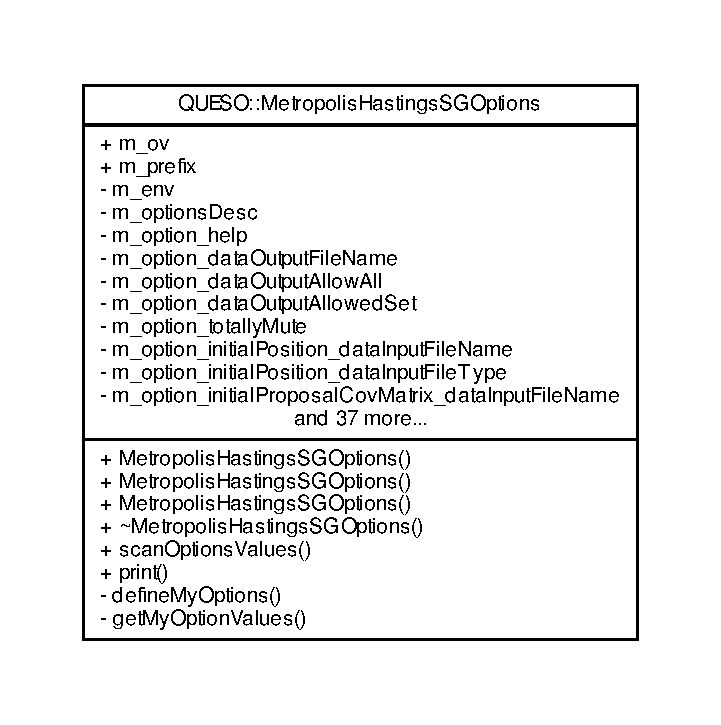
\includegraphics[scale=0.65,clip=true]{rawfigs/metropolis_hastings_options}
% \vspace{-1.2cm}
% \caption{The Metropolis-Hastings sequence generator options class.}
% \label{fig-metropolis-hastings-options-class}
% \end{figure}


\begin{figure}[p]
\centering
% 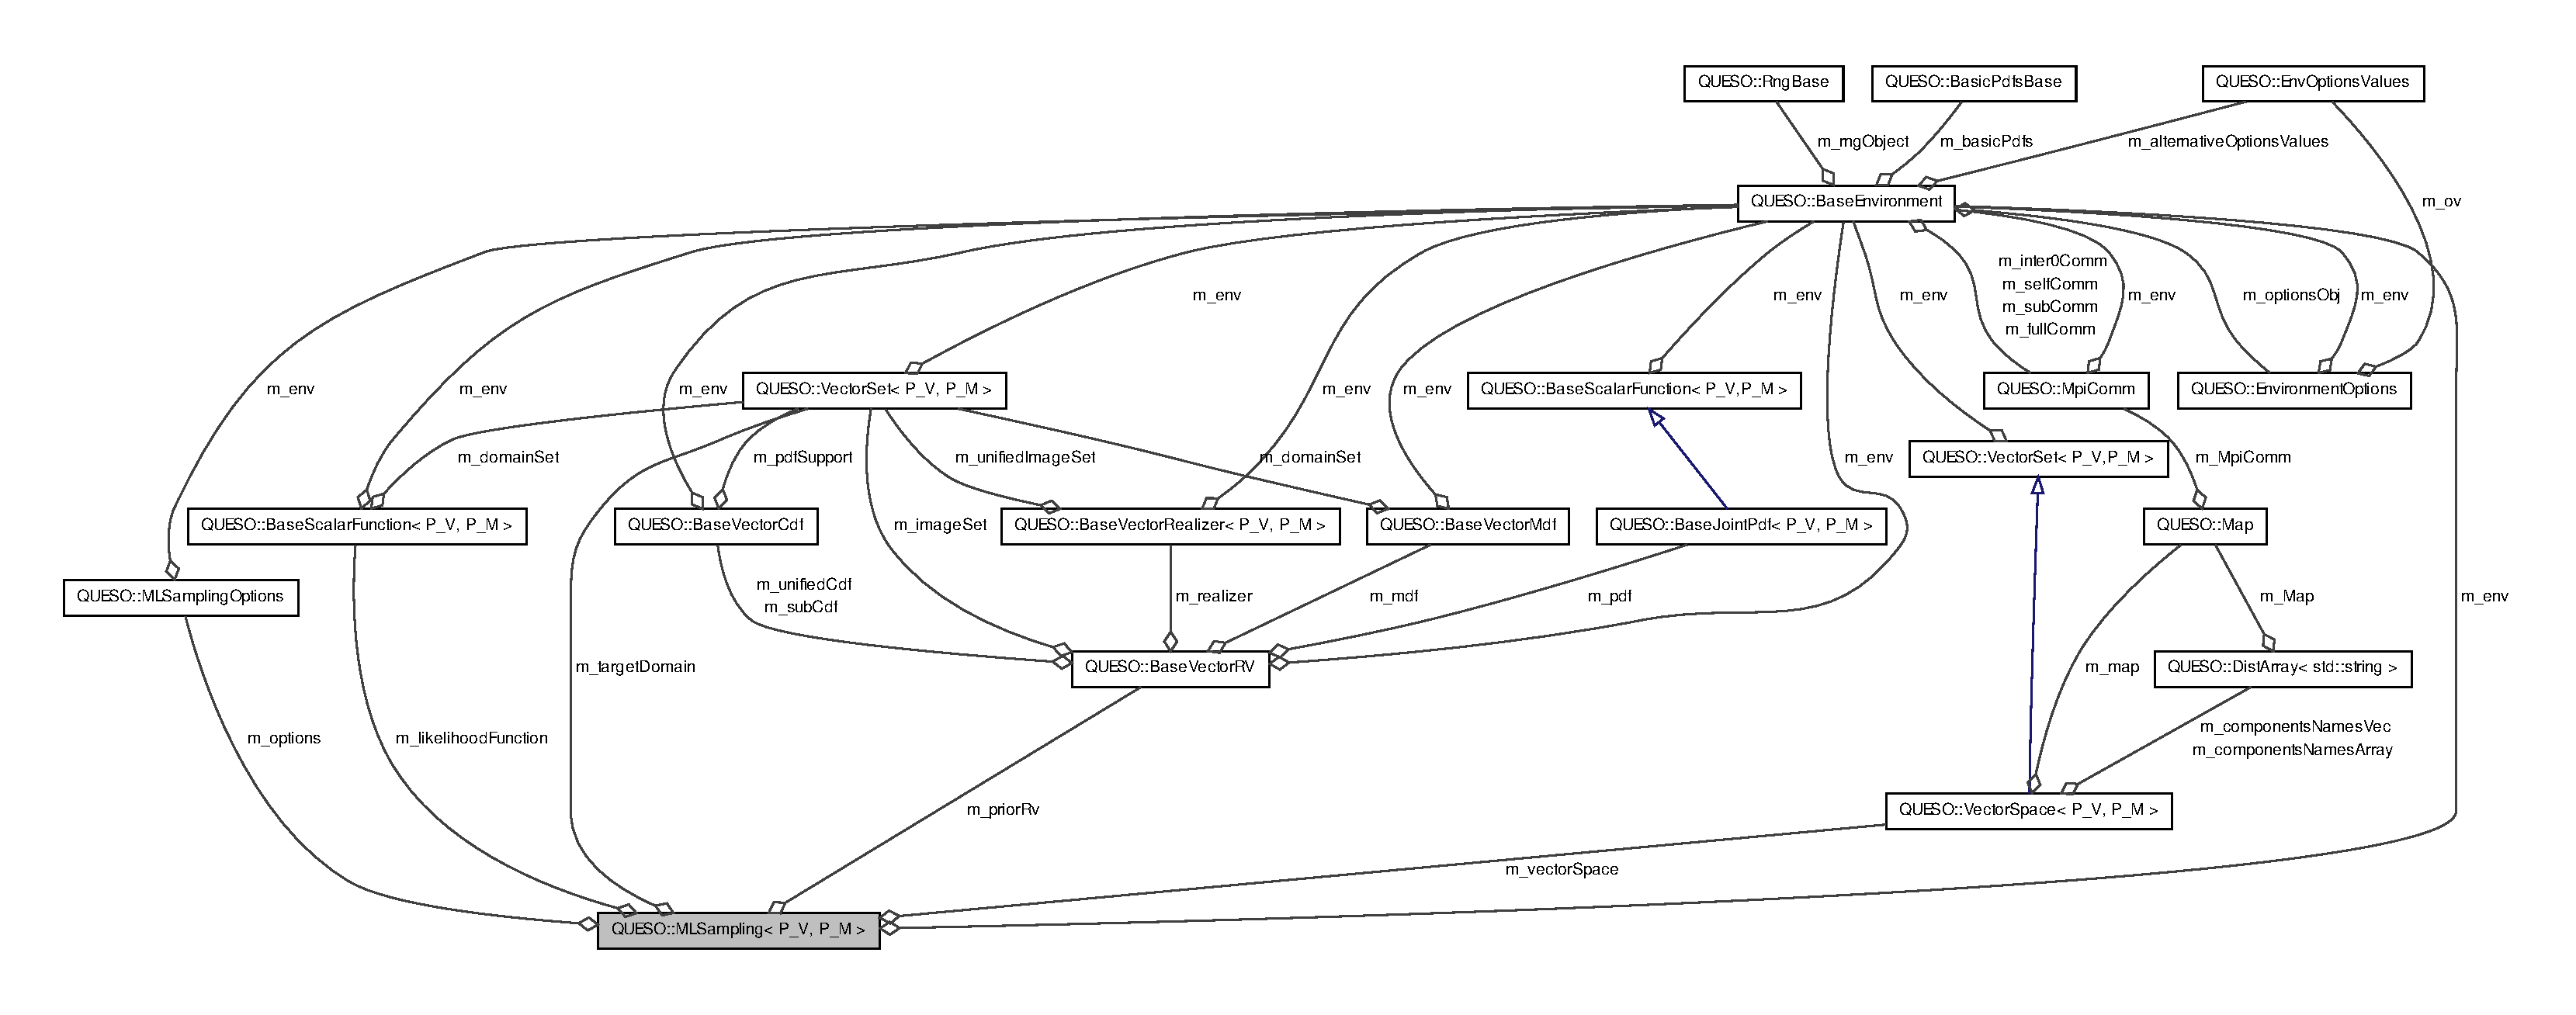
\includegraphics[width=1.3\textwidth, height=.7\textheight,clip=true,angle=90]{rawfigs/ml_coll}
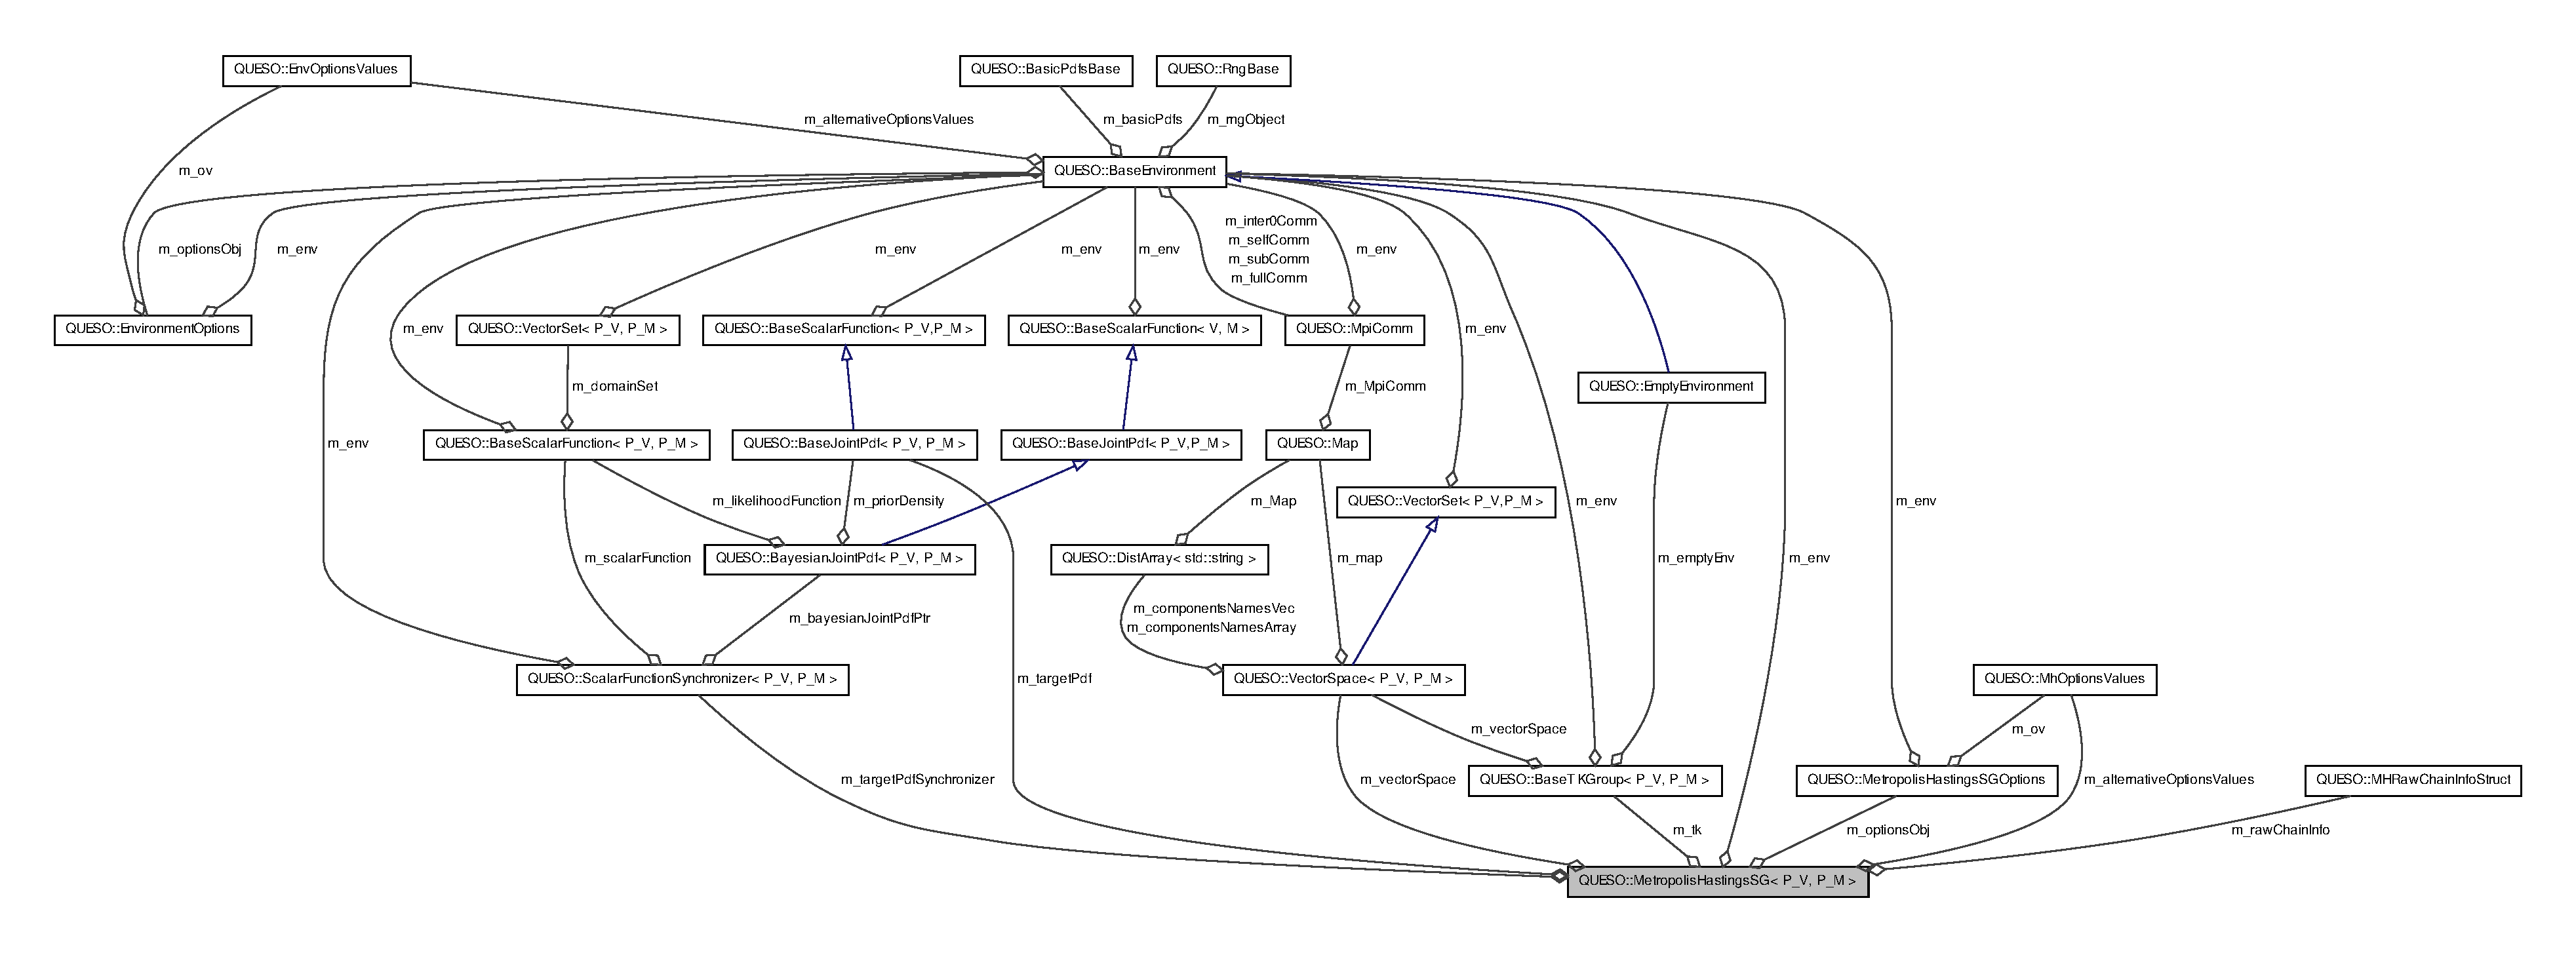
\includegraphics[scale=.35,clip=true,angle=90]{rawfigs/metropolis_hastings_coll}
 \vspace{-.8cm}
\caption{Collaboration graph of the  Metropolis-Hastings sequence generator class.}
\label{fig-metropolis-hastings-coll}
\end{figure}

\begin{table}[htpb]
\begin{center}
\caption{Input file options for a QUESO Metropolis-Hastings solver.}\label{tab-metropolis-hastings-options}
\vspace*{-8pt}
\ttfamily\footnotesize
\begin{tabular}{l c} %  m{4cm}}
\toprule
\rmfamily Option Name                                    & \rmfamily Default Value \\%& \rmfamily Description \\ %
\midrule\midrule
 \textlangle PREFIX\textrangle mh\_dataOutputFileName                       & "."   \\ % (UQ_MH_SG_DATA_OUTPUT_FILE_NAME_ODV),
 \textlangle PREFIX\textrangle mh\_dataOutputAllowAll                       & 0     \\ % (UQ_MH_SG_DATA_OUTPUT_ALLOW_ALL_ODV),
 \textlangle PREFIX\textrangle mh\_initialPositionDataInputFileName         & "."   \\ % (UQ_MH_SG_INITIAL_POSITION_DATA_INPUT_FILE_NAME_ODV),
 \textlangle PREFIX\textrangle mh\_initialPositionDataInputFileType         & "m"   \\ % (UQ_MH_SG_INITIAL_POSITION_DATA_INPUT_FILE_TYPE_ODV),
 \textlangle PREFIX\textrangle mh\_initialProposalCovMatrixDataInputFileName& "."   \\ % (UQ_MH_SG_INITIAL_PROPOSAL_COV_MATRIX_DATA_INPUT_FILE_NAME_ODV),
 \textlangle PREFIX\textrangle mh\_initialProposalCovMatrixDataInputFileType& "m"   \\ % (UQ_MH_SG_INITIAL_PROPOSAL_COV_MATRIX_DATA_INPUT_FILE_TYPE_ODV),
 \textlangle PREFIX\textrangle mh\_rawChainDataInputFileName                & "."   \\ % (UQ_MH_SG_RAW_CHAIN_DATA_INPUT_FILE_NAME_ODV),
 \textlangle PREFIX\textrangle mh\_rawChainDataInputFileType                & "m"   \\ % (UQ_MH_SG_RAW_CHAIN_DATA_INPUT_FILE_TYPE_ODV),
 \textlangle PREFIX\textrangle mh\_rawChainSize                             & 100   \\ % (UQ_MH_SG_RAW_CHAIN_SIZE_ODV),
 \textlangle PREFIX\textrangle mh\_rawChainGenerateExtra                    &  0    \\ % (UQ_MH_SG_RAW_CHAIN_GENERATE_EXTRA_ODV),
 \textlangle PREFIX\textrangle mh\_rawChainDisplayPeriod                    & 500   \\ % (UQ_MH_SG_RAW_CHAIN_DISPLAY_PERIOD_ODV),
 \textlangle PREFIX\textrangle mh\_rawChainMeasureRunTimes                  &  1    \\ % (UQ_MH_SG_RAW_CHAIN_MEASURE_RUN_TIMES_ODV),
 \textlangle PREFIX\textrangle mh\_rawChainDataOutputPeriod                 &  0    \\ % (UQ_MH_SG_RAW_CHAIN_DATA_OUTPUT_PERIOD_ODV),
 \textlangle PREFIX\textrangle mh\_rawChainDataOutputFileName               & "."   \\ % (UQ_MH_SG_RAW_CHAIN_DATA_OUTPUT_FILE_NAME_ODV),
 \textlangle PREFIX\textrangle mh\_rawChainDataOutputFileType               & "m"   \\ % (UQ_MH_SG_RAW_CHAIN_DATA_OUTPUT_FILE_TYPE_ODV),
 \textlangle PREFIX\textrangle mh\_rawChainDataOutputAllowAll               &  0    \\ % (UQ_MH_SG_RAW_CHAIN_DATA_OUTPUT_ALLOW_ALL_ODV),
 \textlangle PREFIX\textrangle mh\_filteredChainGenerate                    &  0    \\ % (UQ_MH_SG_FILTERED_CHAIN_GENERATE_ODV),
 \textlangle PREFIX\textrangle mh\_filteredChainDiscardedPortion            &  0.   \\ % (UQ_MH_SG_FILTERED_CHAIN_DISCARDED_PORTION_ODV),
 \textlangle PREFIX\textrangle mh\_filteredChainLag                         &  1    \\ % (UQ_MH_SG_FILTERED_CHAIN_LAG_ODV),
 \textlangle PREFIX\textrangle mh\_filteredChainDataOutputFileName          & "."   \\ % (UQ_MH_SG_FILTERED_CHAIN_DATA_OUTPUT_FILE_NAME_ODV),
 \textlangle PREFIX\textrangle mh\_filteredChainDataOutputFileType          & "m"   \\ % (UQ_MH_SG_FILTERED_CHAIN_DATA_OUTPUT_FILE_TYPE_ODV),
 \textlangle PREFIX\textrangle mh\_filteredChainDataOutputAllowAll          &  0   \\ % (UQ_MH_SG_FILTERED_CHAIN_DATA_OUTPUT_ALLOW_ALL_ODV),
 \textlangle PREFIX\textrangle mh\_displayCandidates                        &  0    \\ % (UQ_MH_SG_DISPLAY_CANDIDATES_ODV),
 \textlangle PREFIX\textrangle mh\_putOutOfBoundsInChain                    &  1    \\ % (UQ_MH_SG_PUT_OUT_OF_BOUNDS_IN_CHAIN_ODV),
 \textlangle PREFIX\textrangle mh\_tkUseLocalHessian                        &  0    \\ % (UQ_MH_SG_TK_USE_LOCAL_HESSIAN_ODV),
 \textlangle PREFIX\textrangle mh\_tkUseNewtonComponent                     &  1    \\ % (UQ_MH_SG_TK_USE_NEWTON_COMPONENT_ODV),
 \textlangle PREFIX\textrangle mh\_drMaxNumExtraStages                      &  0    \\ % (UQ_MH_SG_DR_MAX_NUM_EXTRA_STAGES_ODV),
%\textlangle PREFIX\textrangle mh\_drScalesForExtraStages                   &    \\ % (0),
 \textlangle PREFIX\textrangle mh\_drDuringAmNonAdaptiveInt                 &  1    \\ % (UQ_MH_SG_DR_DURING_AM_NON_ADAPTIVE_INT_ODV),
 \textlangle PREFIX\textrangle mh\_amKeepInitialMatrix                      &  0    \\ % (UQ_MH_SG_AM_KEEP_INITIAL_MATRIX_ODV),
 \textlangle PREFIX\textrangle mh\_amInitialNonAdaptInterval                &  0    \\ % (UQ_MH_SG_AM_INIT_NON_ADAPT_INT_ODV),
 \textlangle PREFIX\textrangle mh\_amAdaptInterval                          &  0    \\ % (UQ_MH_SG_AM_ADAPT_INTERVAL_ODV),
 \textlangle PREFIX\textrangle mh\_amAdaptedMatricesDataOutputPeriod        &  0    \\ % (UQ_MH_SG_AM_ADAPTED_MATRICES_DATA_OUTPUT_PERIOD_ODV),
 \textlangle PREFIX\textrangle mh\_amAdaptedMatricesDataOutputFileName      & "."   \\ % (UQ_MH_SG_AM_ADAPTED_MATRICES_DATA_OUTPUT_FILE_NAME_ODV),
 \textlangle PREFIX\textrangle mh\_amAdaptedMatricesDataOutputFileType      & "m"   \\ % (UQ_MH_SG_AM_ADAPTED_MATRICES_DATA_OUTPUT_FILE_TYPE_ODV),
 \textlangle PREFIX\textrangle mh\_amAdaptedMatricesDataOutputAllowAll      &  0    \\ % (UQ_MH_SG_AM_ADAPTED_MATRICES_DATA_OUTPUT_ALLOW_ALL_ODV),
%\textlangle PREFIX\textrangle mh\_amAdaptedMatricesDataOutputAllowedSet    &    \\ % (),
 \textlangle PREFIX\textrangle mh\_amEta                                    & 1.    \\ % (UQ_MH_SG_AM_ETA_ODV),
 \textlangle PREFIX\textrangle mh\_amEpsilon                                & $1\times 10^{-5}$   \\ % (UQ_MH_SG_AM_EPSILON_ODV),
 \textlangle PREFIX\textrangle mh\_enableBrooksGelmanConvMonitor            & 0    \\ % (UQ_MH_SG_ENABLE_BROOKS_GELMAN_CONV_MONITOR),
 \textlangle PREFIX\textrangle mh\_BrooksGelmanLag                          & 100   \\ % (UQ_MH_SG_BROOKS_GELMAN_LAG)
\bottomrule
\end{tabular}
\end{center}
\end{table}




%\clearpage
\subsection{Multilevel Solver (and Options)}\label{sec:ML}


The templated class that represents a Multilevel generator of samples in QUESO is \linebreak \verb+MLSampling<P_V,P_M>+. This class implements the Adaptive Multilevel Stochastic Simulation Algorithm of Cheung and Prudencio~\cite{CheungPrudencio2012}.
The Multilevel sequence generator class is assisted by two extra classes, \verb+MLSamplingOptions+ and \verb+MLSamplingLevelOptions+, for handling the options to be used.

The Multilevel class, the Multilevel options and level options classes are depicted in Figure~\ref{fig-Multilevel-options-class}.  A collaboration graph for the Multilevel class is presented in Figure \ref{fig-Multilevel-coll}; whereas its associated options are presented in Table \ref{tab-Multilevel-options}.
% 
% \begin{figure}[htpb]
% \centering
% 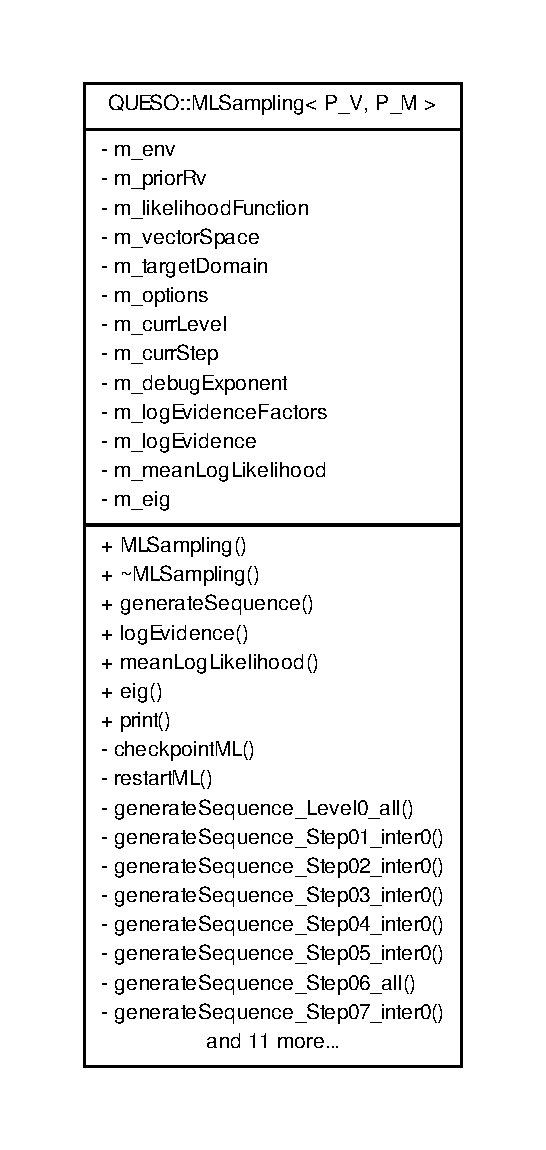
\includegraphics[scale=0.8,clip=true]{rawfigs/ml_sampling}
% \vspace{-1.cm}
% \caption{The Multilevel sequence generator class.}
% \label{fig-Multilevel-solver-class}
% \end{figure}

\begin{figure}[htpb]
\centering
\subfloat[MLSampling]{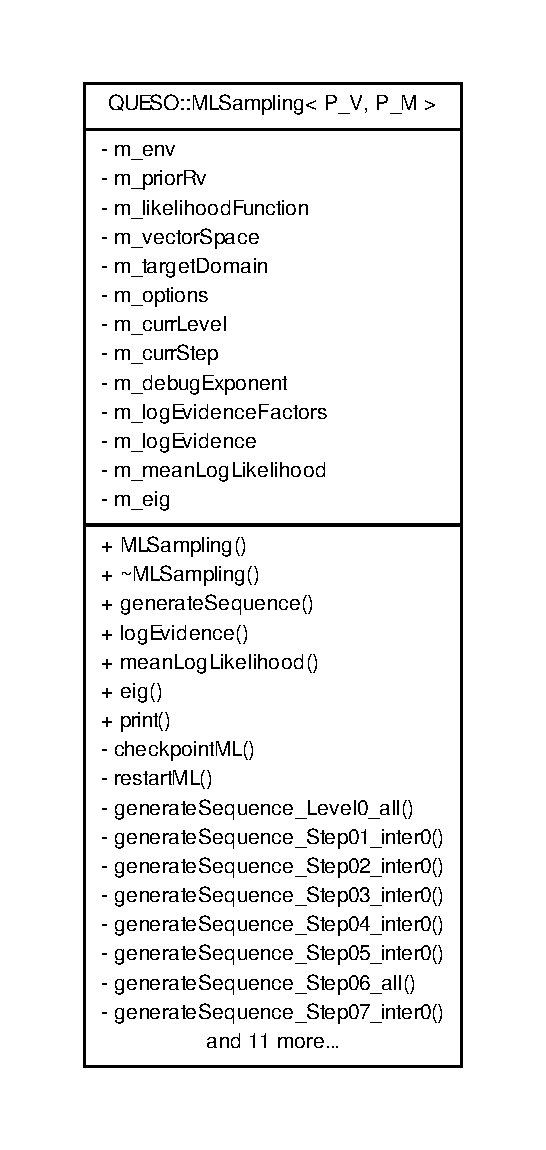
\includegraphics[trim={0 1.3cm 0 0},clip,scale=0.65]{rawfigs/ml_sampling}\label{fig-Multilevel-solver-class}}\hspace{-1.5cm}
\subfloat[MLSamplingOptions]{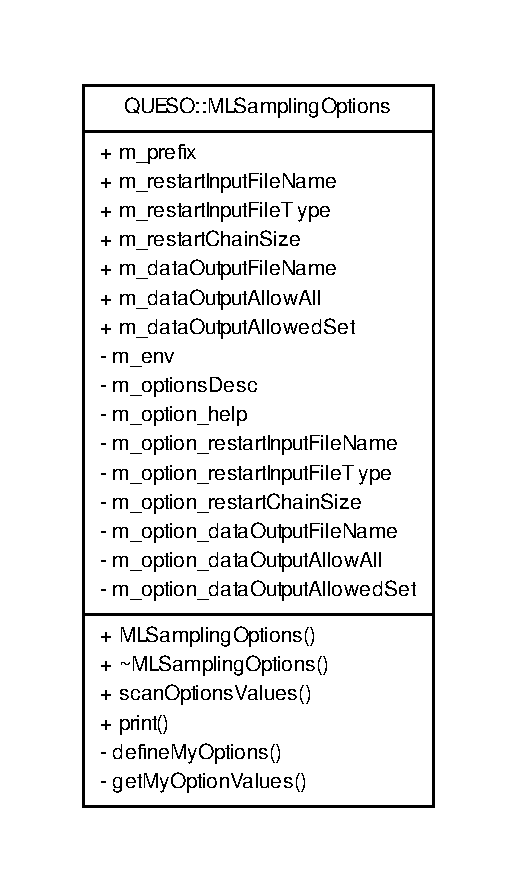
\includegraphics[trim={0 1.3cm 0 0},clip,scale=0.65]{rawfigs/ml_sampling_options}}\hspace{-1.5cm}
\subfloat[MLSamplingLevelOptions]{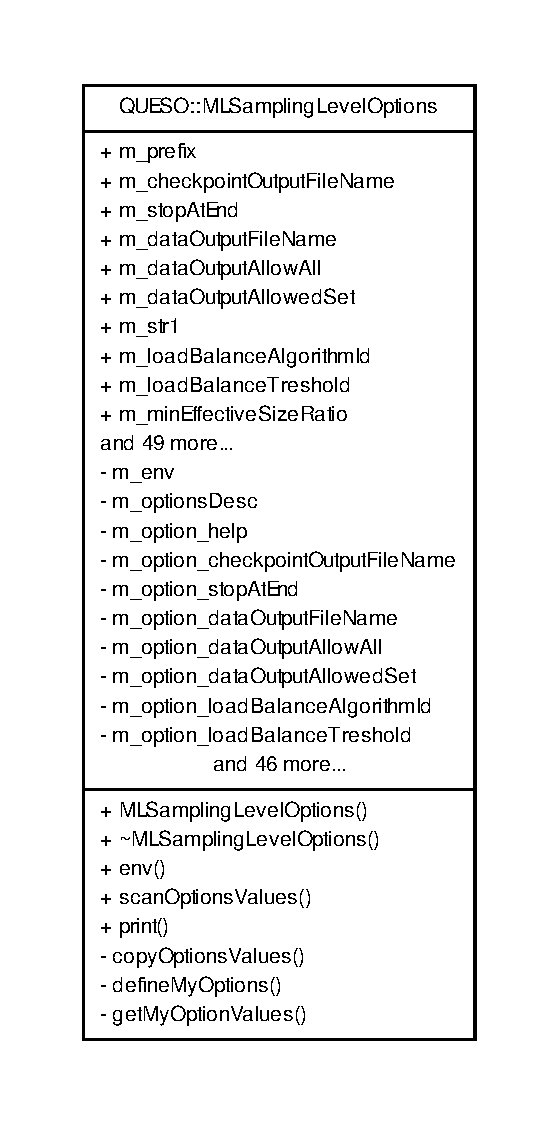
\includegraphics[trim={0 1.3cm 0 0},clip,scale=0.65]{rawfigs/ml_sampling_level_options}}
 \vspace{-.2cm}
\caption{The Multilevel sequence generator options class (\ref{fig-Multilevel-solver-class}) and its associated classes for handling options.}
\label{fig-Multilevel-options-class}
\end{figure}


\begin{figure}[p]
\centering
% 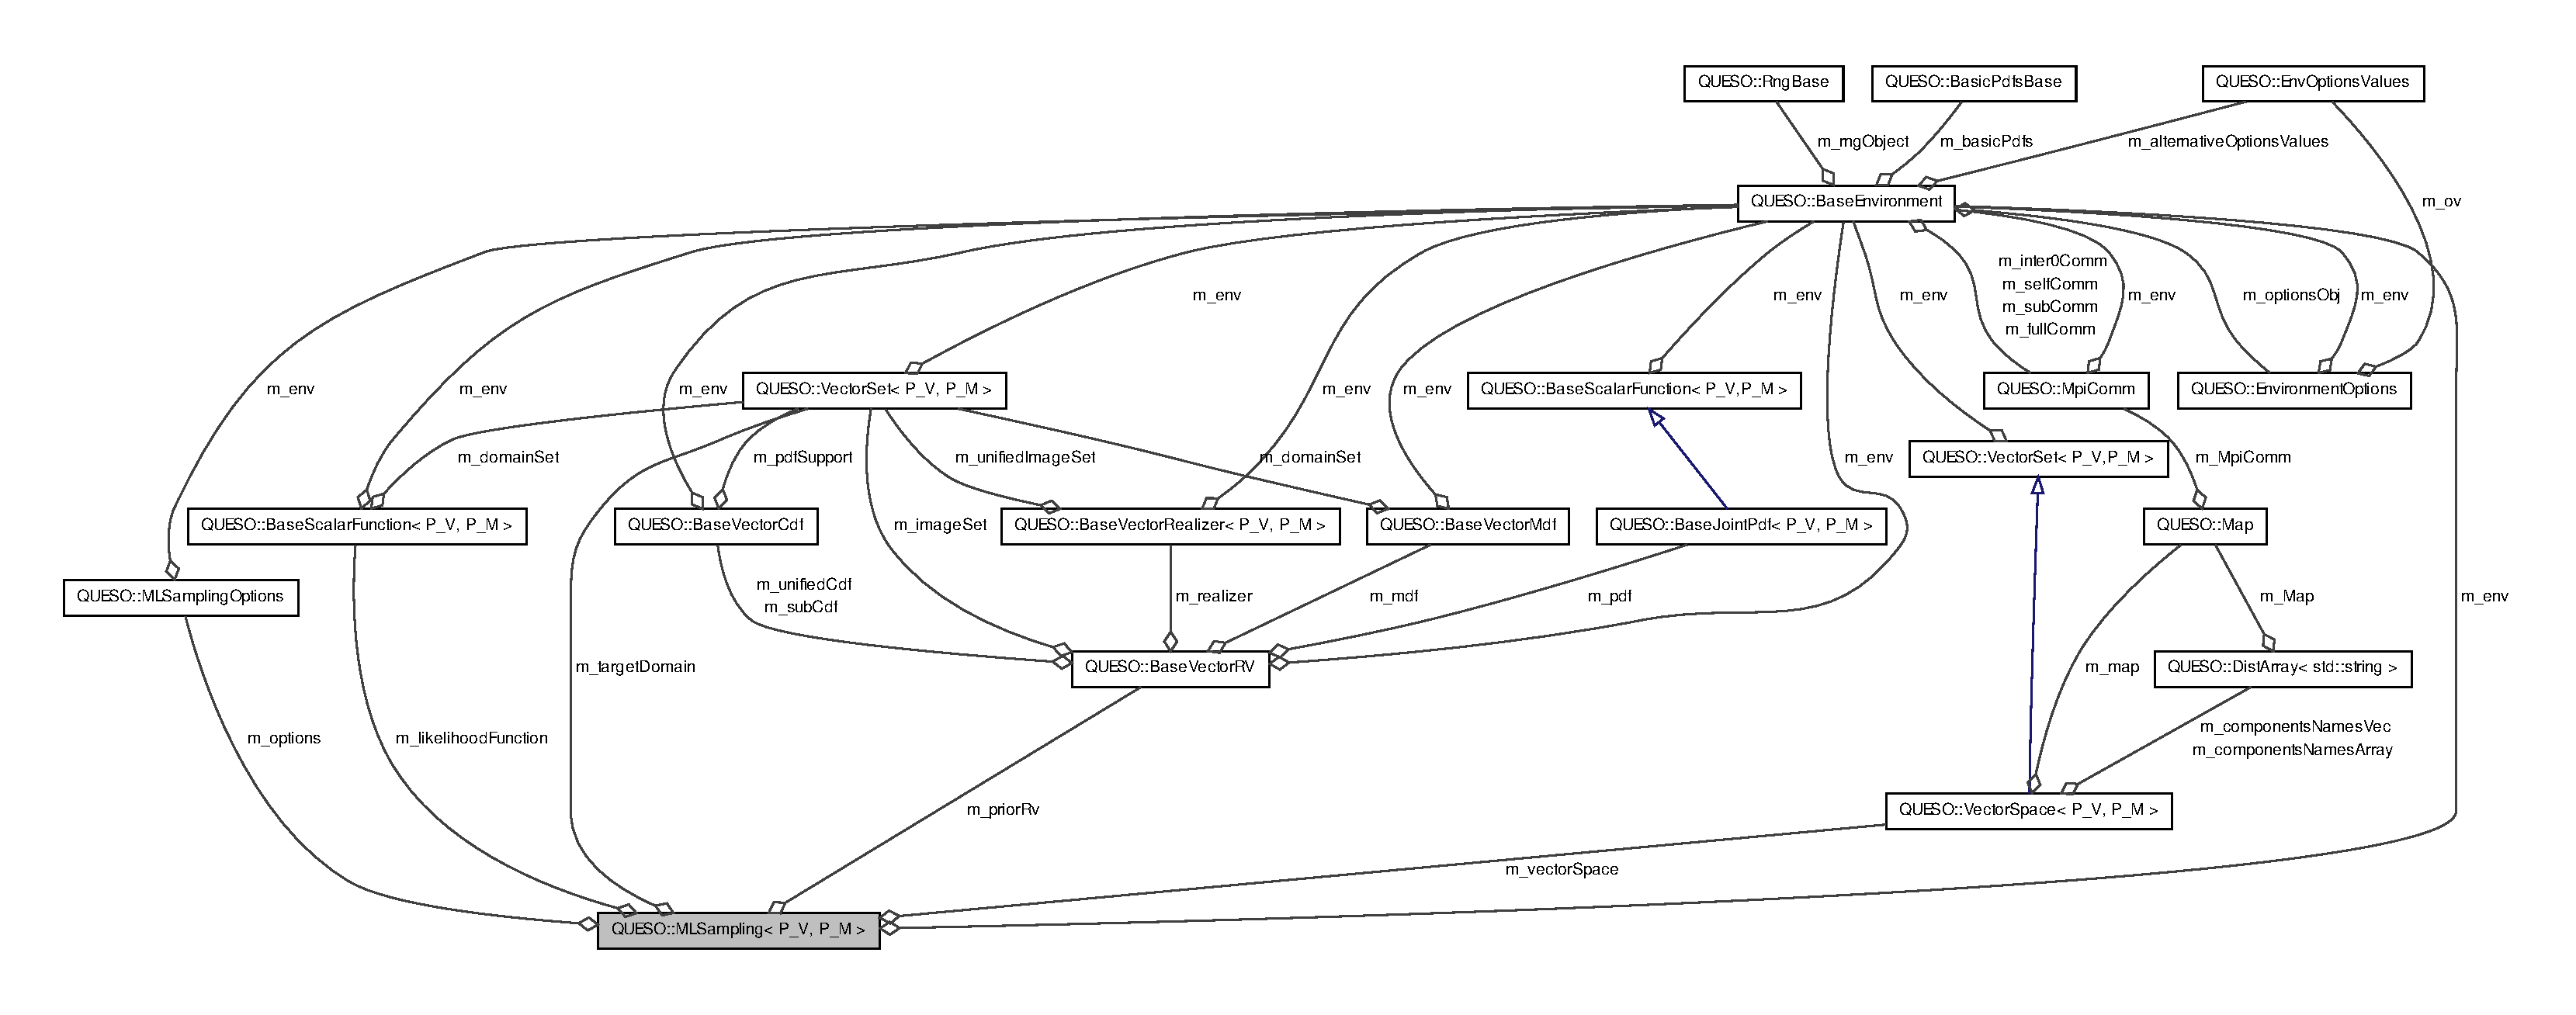
\includegraphics[width=1.3\textwidth, height=.7\textheight,clip=true,angle=90]{rawfigs/ml_coll}
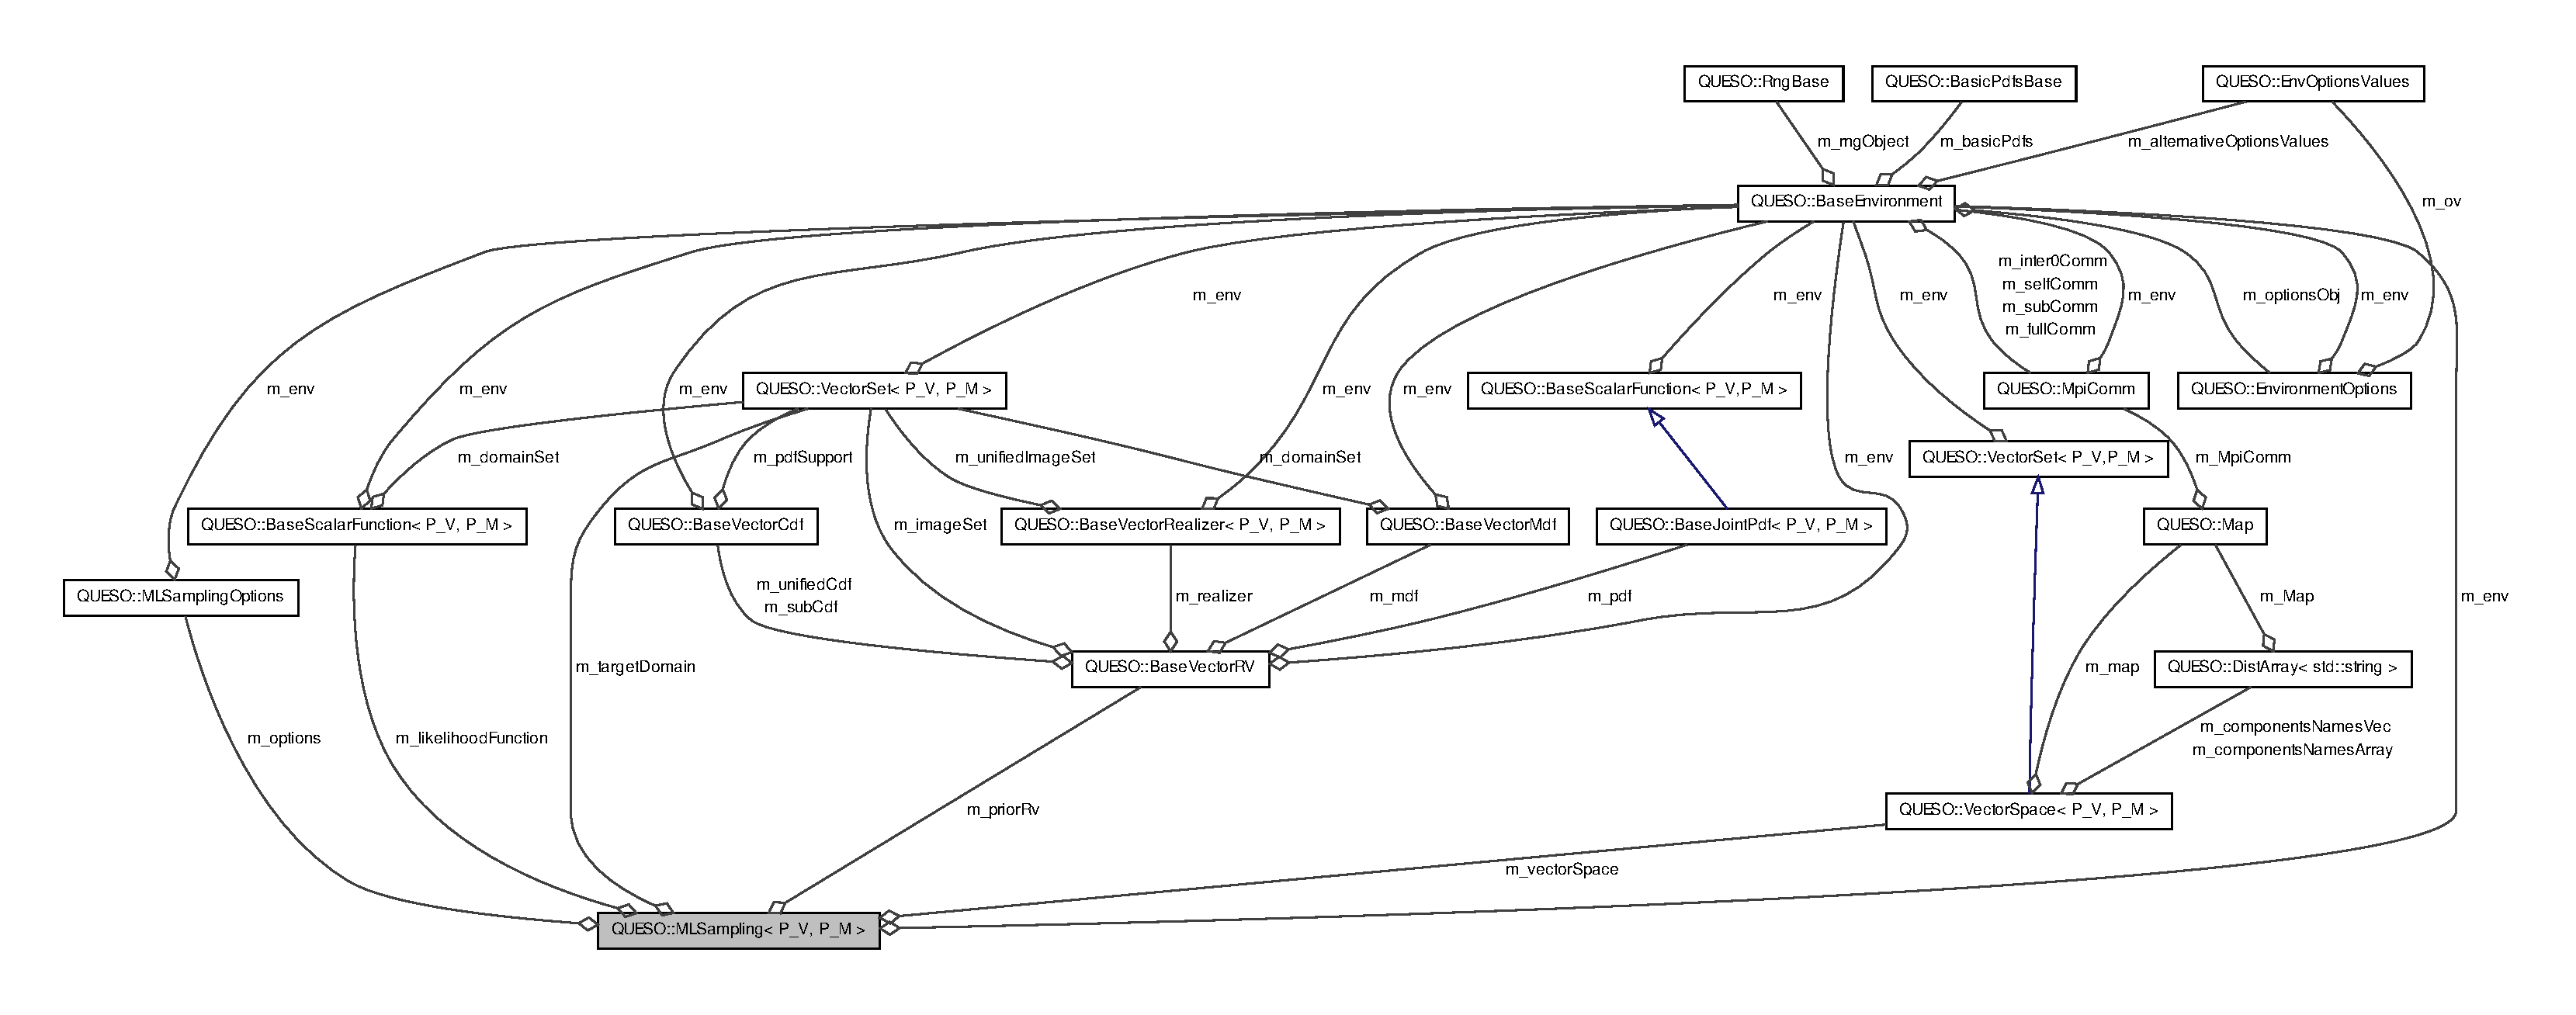
\includegraphics[scale=.4,clip=true,angle=90]{rawfigs/ml_coll}
 \vspace{-.8cm}
\caption{Collaboration graph of the  Multilevel sampling class.}
\label{fig-Multilevel-coll}
\end{figure}


\begin{table}[p]
\begin{center}
\caption{Input file options for a QUESO Multilevel solver (to be continued).}\label{tab-Multilevel-options}
\vspace*{-8pt}
\ttfamily\footnotesize
\begin{tabular}{l c} %  m{4cm}}
\toprule
\rmfamily Option Name                                    & \rmfamily Default Value \\%& \rmfamily Description \\ %
\midrule\midrule
% \textlangle PREFIX\textrangle
% ml\_dataOutputFileName              & "."  \\ %  (UQ_ML_SAMPLING_DATA_Output\_FILE_NAME_ODV  )

\textlangle PREFIX\textrangle
ml\_restartOutput\_levelPeriod       & 0    \\ %  (UQ_ML_SAMPLING_RESTART_Output\_LEVEL_PERIOD_ODV       ),

\textlangle PREFIX\textrangle 
ml\_restartOutput\_baseNameForFiles  & "."  \\ %  (UQ_ML_SAMPLING_RESTART_Output\_BASE_NAME_FOR_FILES_ODV),

\textlangle PREFIX\textrangle 
ml\_restartOutput\_fileType          & "m"  \\ %  (UQ_ML_SAMPLING_RESTART_Output\_FILE_TYPE_ODV          ),

\textlangle PREFIX\textrangle 
ml\_restartInput\_baseNameForFiles   & "."  \\ %  (UQ_ML_SAMPLING_RESTART_Input\_BASE_NAME_FOR_FILES_ODV ),

\textlangle PREFIX\textrangle 
ml\_restartInput\_fileType           & "m"  \\ %  (UQ_ML_SAMPLING_RESTART_Input\_FILE_TYPE_ODV           ),

% \textlangle PREFIX\textrangle ml\_option\_dataOutputAllowedSet   & ""  \\ %  (\textlangle PREFIX\textrangle ml\_prefix + "dataOutputAllowedSet")

 \textlangle PREFIX\textrangle ml\_stopAtEnd                                 & 0    \\%  (UQ_ML_SAMPLING_L_STOP_AT_END_ODV),
 \textlangle PREFIX\textrangle ml\_dataOutputFileName                        & "."  \\%  (UQ_ML_SAMPLING_L_DATA_OUTPUT_FILE_NAME_ODV),
 \textlangle PREFIX\textrangle ml\_dataOutputAllowAll                        & 0    \\%  (UQ_ML_SAMPLING_L_DATA_OUTPUT_ALLOW_ALL_ODV),
 \textlangle PREFIX\textrangle ml\_loadBalanceAlgorithmId                    & 2    \\%  (UQ_ML_SAMPLING_L_LOAD_BALANCE_ALGORITH),
 \textlangle PREFIX\textrangle ml\_loadBalanceTreshold                       & 1.0  \\%  (UQ_ML_SAMPLING_L_LOAD_BALANCE_TRESHOLD_ODV),
 \textlangle PREFIX\textrangle ml\_minEffectiveSizeRatio                     & 0.85 \\%  (UQ_ML_SAMPLING_L_MIN_EFFECTIVE_SIZE_RATIO_ODV),
 \textlangle PREFIX\textrangle ml\_maxEffectiveSizeRatio                     & 0.91 \\%  (UQ_ML_SAMPLING_L_MAX_EFFECTIVE_SIZE_RATIO_ODV),
 \textlangle PREFIX\textrangle ml\_scaleCovMatrix                            & 1    \\%  (UQ_ML_SAMPLING_L_SCALE_COV_MATRIX_ODV),
 \textlangle PREFIX\textrangle ml\_minRejectionRate                          & 0.50 \\%  (UQ_ML_SAMPLING_L_MIN_REJECTION_RATE_ODV),
 \textlangle PREFIX\textrangle ml\_maxRejectionRate                          & 0.75 \\%  (UQ_ML_SAMPLING_L_MAX_REJECTION_RATE_ODV),
 \textlangle PREFIX\textrangle ml\_covRejectionRate                          & 0.25 \\%  (UQ_ML_SAMPLING_L_COV_REJECTION_RATE_ODV),
 \textlangle PREFIX\textrangle ml\_minAcceptableEta                          & 0.   \\%  (UQ_ML_SAMPLING_L_MIN_ACCEPTABLE_ETA_ODV), // gpmsa
 \textlangle PREFIX\textrangle ml\_totallyMute                               & 1    \\%  (UQ_ML_SAMPLING_L_TOTALLY_MUTE_ODV),
 \textlangle PREFIX\textrangle ml\_initialPositionDataInputFileName          & "."  \\%  (UQ_ML_SAMPLING_L_INITIAL_POSITION_DATA_INPUT_FILE_NAME_ODV),
 \textlangle PREFIX\textrangle ml\_initialPositionDataInputFileType          & "m"  \\%  (UQ_ML_SAMPLING_L_INITIAL_POSITION_DATA_INPUT_FILE_TYPE_ODV),
 \textlangle PREFIX\textrangle ml\_initialProposalCovMatrixDataInputFileName & "."  \\%  (UQ_ML_SAMPLING_L_INITIAL_PROPOSAL_COV_MATRIX_DATA_INPUT_FILE_NAME_ODV),
 \textlangle PREFIX\textrangle ml\_initialProposalCovMatrixDataInputFileType & "m"  \\%  (UQ_ML_SAMPLING_L_INITIAL_PROPOSAL_COV_MATRIX_DATA_INPUT_FILE_TYPE_ODV),
 \textlangle PREFIX\textrangle ml\_rawChainDataInputFileName                 & "."  \\%  (UQ_ML_SAMPLING_L_RAW_CHAIN_DATA_INPUT_FILE_NAME_ODV),
 \textlangle PREFIX\textrangle ml\_rawChainDataInputFileType                 & "m"  \\%  (UQ_ML_SAMPLING_L_RAW_CHAIN_DATA_INPUT_FILE_TYPE_ODV),
 \textlangle PREFIX\textrangle ml\_rawChainSize                              & 100  \\%  (UQ_ML_SAMPLING_L_RAW_CHAIN_SIZE_ODV),
 \textlangle PREFIX\textrangle ml\_rawChainGenerateExtra                     & 0    \\%  (UQ_ML_SAMPLING_L_RAW_CHAIN_GENERATE_EXTRA_ODV),
 \textlangle PREFIX\textrangle ml\_rawChainDisplayPeriod                     & 500  \\%  (UQ_ML_SAMPLING_L_RAW_CHAIN_DISPLAY_PERIOD_ODV),
 \textlangle PREFIX\textrangle ml\_rawChainMeasureRunTimes                   & 1    \\%  (UQ_ML_SAMPLING_L_RAW_CHAIN_MEASURE_RUN_TIMES_ODV),
 \textlangle PREFIX\textrangle ml\_rawChainDataOutputPeriod                  & 0    \\%  (UQ_ML_SAMPLING_L_RAW_CHAIN_DATA_OUTPUT_PERIOD_ODV),
 \textlangle PREFIX\textrangle ml\_rawChainDataOutputFileName                & "."  \\%  (UQ_ML_SAMPLING_L_RAW_CHAIN_DATA_OUTPUT_FILE_NAME_ODV),
 \textlangle PREFIX\textrangle ml\_rawChainDataOutputFileType                & "m"  \\%  (UQ_ML_SAMPLING_L_RAW_CHAIN_DATA_OUTPUT_FILE_TYPE_ODV),
 \textlangle PREFIX\textrangle ml\_rawChainDataOutputAllowAll                & 0    \\%  (UQ_ML_SAMPLING_L_RAW_CHAIN_DATA_OUTPUT_ALLOW_ALL_ODV),
 \textlangle PREFIX\textrangle ml\_filteredChainGenerate                     & 0    \\%  (UQ_ML_SAMPLING_L_FILTERED_CHAIN_GENERATE_ODV),
 \textlangle PREFIX\textrangle ml\_filteredChainDiscardedPortion             & 0.   \\%  (UQ_ML_SAMPLING_L_FILTERED_CHAIN_DISCARDED_PORTION_ODV),
 \textlangle PREFIX\textrangle ml\_filteredChainLag                          & 1    \\%  (UQ_ML_SAMPLING_L_FILTERED_CHAIN_LAG_ODV),
 \textlangle PREFIX\textrangle ml\_filteredChainDataOutputFileName           & "."  \\%  (UQ_ML_SAMPLING_L_FILTERED_CHAIN_DATA_OUTPUT_FILE_NAME_ODV),
 \textlangle PREFIX\textrangle ml\_filteredChainDataOutputFileType           & "m"  \\%  (UQ_ML_SAMPLING_L_FILTERED_CHAIN_DATA_OUTPUT_FILE_TYPE_ODV),
 \textlangle PREFIX\textrangle ml\_filteredChainDataOutputAllowAll           & 0    \\%  (UQ_ML_SAMPLING_L_FILTERED_CHAIN_DATA_OUTPUT_ALLOW_ALL_ODV),
 \textlangle PREFIX\textrangle ml\_displayCandidates                         & 0    \\%  (UQ_ML_SAMPLING_L_DISPLAY_CANDIDATES_ODV),
 \textlangle PREFIX\textrangle ml\_putOutOfBoundsInChain                     & 1    \\%  (UQ_ML_SAMPLING_L_PUT_OUT_OF_BOUNDS_IN_CHAIN_ODV),

 \textlangle PREFIX\textrangle ml\_tkUseLocalHessian                         & 0    \\%  (UQ_ML_SAMPLING_L_TK_USE_LOCAL_HESSIAN_ODV),
 \textlangle PREFIX\textrangle ml\_tkUseNewtonComponent                      & 1    \\%  (UQ_ML_SAMPLING_L_TK_USE_NEWTON_COMPONENT_ODV),
 \textlangle PREFIX\textrangle ml\_drMaxNumExtraStages                       & 0    \\%  (UQ_ML_SAMPLING_L_DR_MAX_NUM_EXTRA_STAGES_ODV),
 \textlangle PREFIX\textrangle ml\_drScalesForExtraStages                    & 0    \\%  (0),
 \textlangle PREFIX\textrangle ml\_drDuringAmNonAdaptiveInt                  & 1    \\%  (UQ_ML_SAMPLING_L_DR_DURING_AM_NON_ADAPTIVE_INT_ODV),
 \textlangle PREFIX\textrangle ml\_amKeepInitialMatrix                       & 0    \\%  (UQ_ML_SAMPLING_L_AM_KEEP_INITIAL_MATRIX_ODV),
 \textlangle PREFIX\textrangle ml\_amInitialNonAdaptInterval                 & 0    \\%  (UQ_ML_SAMPLING_L_AM_INIT_NON_ADAPT_INT_ODV),
 \textlangle PREFIX\textrangle ml\_amAdaptInterval                           & 0    \\%  (UQ_ML_SAMPLING_L_AM_ADAPT_INTERVAL_ODV),
 \textlangle PREFIX\textrangle ml\_amAdaptedMatricesDataOutputPeriod         & 0    \\%  (UQ_ML_SAMPLING_L_AM_ADAPTED_MATRICES_DATA_OUTPUT_PERIOD_ODV),
 \textlangle PREFIX\textrangle ml\_amAdaptedMatricesDataOutputFileName       & "."  \\ %  (UQ_ML_SAMPLING_L_AM_ADAPTED_MATRICES_DATA_OUTPUT_FILE_NAME_ODV),
 \textlangle PREFIX\textrangle ml\_amAdaptedMatricesDataOutputFileType       & "m"  \\ %  (UQ_ML_SAMPLING_L_AM_ADAPTED_MATRICES_DATA_OUTPUT_FILE_TYPE_ODV),
 \textlangle PREFIX\textrangle ml\_amAdaptedMatricesDataOutputAllowAll       & 0    \\ %  (UQ_ML_SAMPLING_L_AM_ADAPTED_MATRICES_DATA_OUTPUT_ALLOW_ALL_ODV),
 \textlangle PREFIX\textrangle ml\_amEta                                     & 1.   \\ %  (UQ_ML_SAMPLING_L_AM_ETA_ODV),
 \textlangle PREFIX\textrangle ml\_amEpsilon                                 & 1.e-5\\ %  (UQ_ML_SAMPLING_L_AM_EPSILON_ODV),
\bottomrule
\end{tabular}
\end{center}
\end{table}



% 
% \begin{table}[!p]
% \begin{center}
% \caption{Input file options for a QUESO Multilevel solver (continuation of Table \ref{tab-Multilevel-options}).}
% %\vspace*{-8pt}
% \ttfamily\small
% \begin{tabular}{l c} %  m{4cm}}
% \toprule
% \rmfamily Option Name                                    & \rmfamily Default Value \\%& \rmfamily Description \\ %
% \midrule\midrule
% 
% 
% \bottomrule
% \end{tabular}
% \end{center}
% \end{table}


%\clearpage
\subsection{Statistical Forward Problem (and Options)}

A SFP in QUESO also has two input entities, the input (parameter) RV and a QoI function, and one output entity, the QoI RV. 
The SIP is represented through the templated class \verb+StatisticalForwardProblem<P_V,P_M,Q_V,Q_M >+, which diagram is presented in Figure \ref{fig-sfp-class}. Again, the types \verb+P_V+ and \verb+Q_V+ of vectors and types \verb+P_M+ and \verb+Q_M+ of matrices, where \verb+P_+ stands for 'parameter' and \verb+Q_+ stands for 'quantities of interest'.

The input RV and the output QoI RV are instances of the \verb+BaseVectorRv<P_V,P_M>+ class, while
the QoI function is an instance of \verb+BaseVectorFunction<P_V,P_M,Q_V,Q_M>+.
In the template parameters, the prefix \verb+P_+ refers to the parameters, whereas the prefix \verb+Q_+ refers to the QoIs.

In order to find the solution of a SFP, one must call the \verb+solveWithMonteCarlo()+ member function of the \verb+StatisticalForwardProblem<P_V,P_M>+ class.
Upon return from a solution operation, the QoI RV is available through the \verb+qoiRv()+ member function. Such QoI RV  is able to provide:
a vector realizer through the operation \verb+'qoiRv().realizer()'+, which returns an instance of the class \verb+'uqBaseVectorRealizer<Q_V,Q_M>'+.



Figure \ref{fig-sfp-options-class} displays the  statistical forward problem options class, i.e. that class that handles a variety of options for solving the SFP. Such options may be provided to QUESO at the user's input file; and they are listed in Table \ref{tab-sfp-options}. In the table, \texttt{p-q} stands for parameter--quantity of interest. 



 
%it provides both CDFs of QoI components through the operation \verb+qoiRv().unifiedCdf()+,  which returns an instance of the class \verb+BaseVectorCdf<Q_V,Q_M>+, and
%a vector realizer through the operation \verb+qoiRv().realizer()+, which returns an instance of the class \verb+BaseVectorRealizer<Q_V,Q_M>+.

\begin{figure}[p]
\centering
\centering
\subfloat[StatisticalForwardProblem]{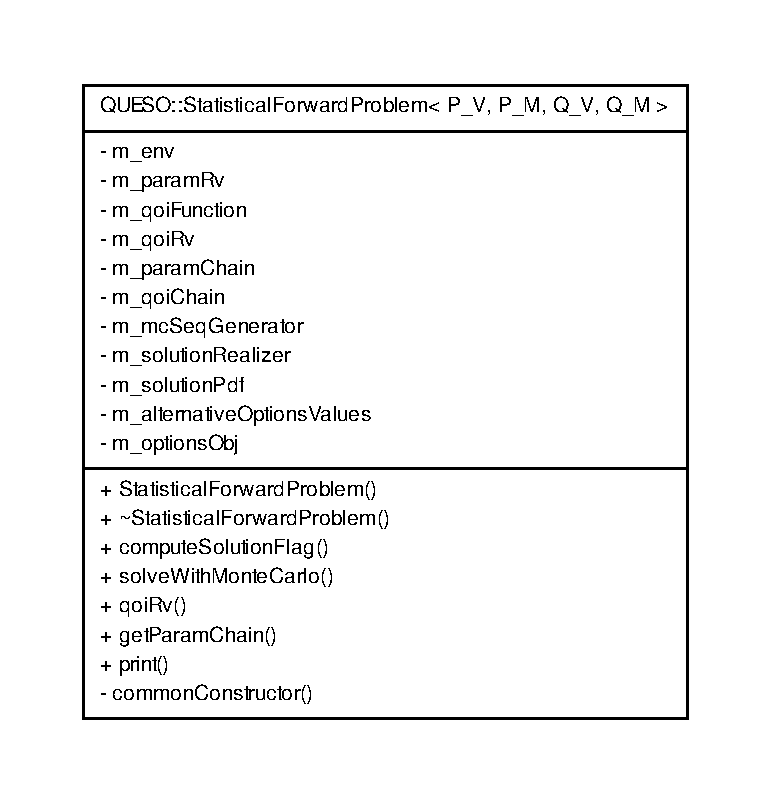
\includegraphics[trim={0.5cm 1.3cm 0 0},clip,scale=0.7]{rawfigs/statistical_forward_problem}\label{fig-sfp-class}}
%
\subfloat[StatisticalForwardProblemOptions]{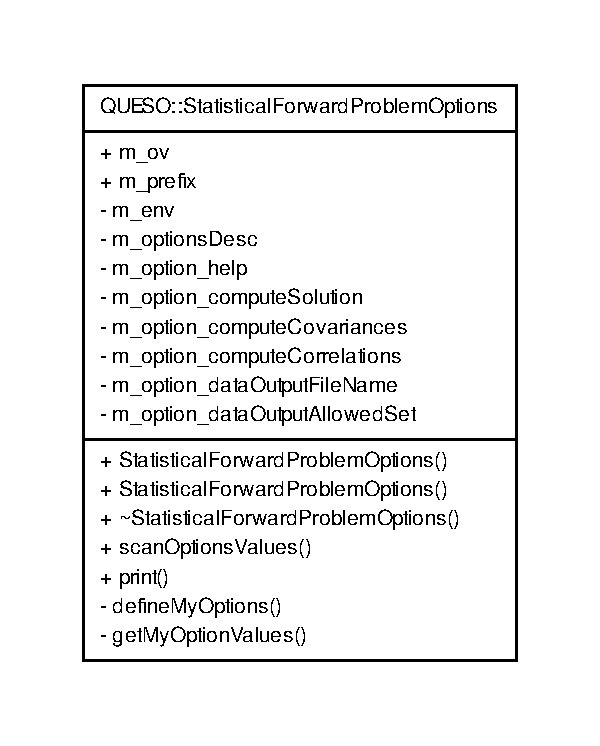
\includegraphics[trim={0.5cm 1.3cm 0 0},clip,scale=0.7]{rawfigs/statistical_forward_problem_options}\label{fig-sfp-options-class}}
\vspace{-.2cm}
%
\caption{The statistical forward problem class, which implements the representation in Figure~\ref{fig-sfp-queso}, and the statistical forward problem options class.}
\end{figure}




\begin{table}[htpb]
% from uqStatisticalForwardProblemOptions.C and .h
\caption{Input file options for a QUESO statistical forward problem.}\label{tab-sfp-options}
\vspace{-8pt}
\ttfamily\footnotesize
\begin{center}
\begin{tabular}{l c  m{6cm}}
\toprule
 \rmfamily Option Name                     & \rmfamily Default Value& \rmfamily Description \\
\midrule
%\textlangle PREFIX\textrangle fp\_help                 &       &             \\ %
%\hline
\textlangle PREFIX\textrangle fp\_computeSolution      &   1  &\rmfamily Computes the solution process   \\%UQ_SFP_COMPUTE_SOLUTION_ODV
%\hline
\textlangle PREFIX\textrangle fp\_computeCovariances   &   1  &\rmfamily Compute \verb+p-q+ covariances    \\ %UQ_SFP_COMPUTE_COVARIANCES_ODV
%\hline
\textlangle PREFIX\textrangle fp\_computeCorrelations  &   1  &\rmfamily Compute \verb+p-q+ correlations   \\ %UQ_SFP_COMPUTE_CORRELATIONS_ODV
%\hline
\textlangle PREFIX\textrangle fp\_dataOutputFileName   &  "." &\rmfamily Name of data output file  \\ %UQ_SFP_DATA_OUTPUT_FILE_NAME_ODV
%\hline
\textlangle PREFIX\textrangle fp\_dataOutputAllowedSet &  ""  &\rmfamily Subenvironments that will write to data output file   \\ %UQ_SFP_DATA_OUTPUT_ALLOWED_SET_ODV
\bottomrule
\end{tabular}
\end{center}
\end{table}

%\clearpage
\subsection{Monte Carlo Solver (and Options)}

The templated class that implements a Monte Carlo generator of samples within QUESO is \verb+MonteCarloSG<P_V,P_M,Q_V,Q_M>+, as illustrated in Figure \ref{fig-monte-carlo-solver-class}.
This class has the requirement that the image set of the vector random variable  and the domain set of the QoI function belong to vector spaces of equal dimensions. If the requirements are satisfied, the class constructor reads input options that begin with the string `\verb+<PREFIX>_mc_+' (See Table~\ref{tab-monte-carlo-options}). Options reading is handled by class \verb+MonteCarloOptions+, which is illustrated in Figure~\ref{fig-monte-carlo-options-class}.


\begin{figure}[p]
\centering
\subfloat[MonteCarloSG]{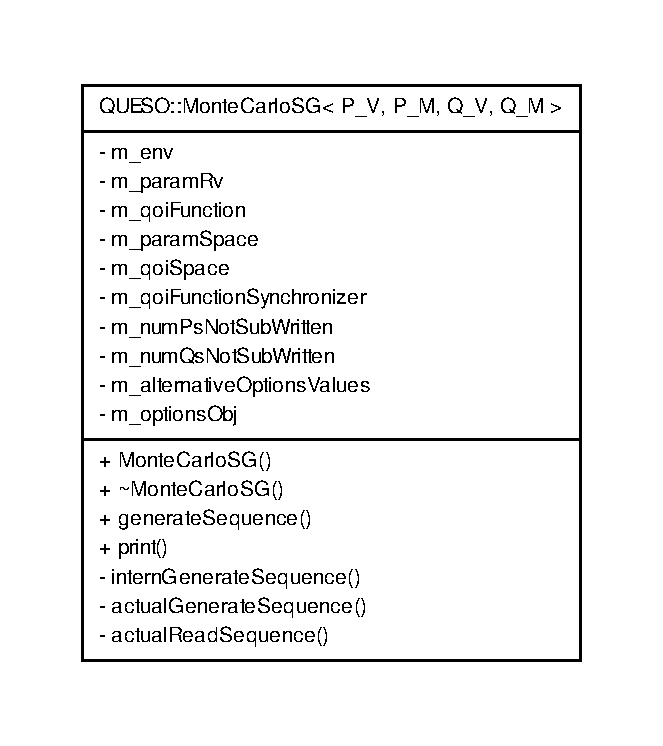
\includegraphics[trim={0.5cm 1.3cm 0 0},clip,scale=0.7]{rawfigs/monte_carlo}\label{fig-monte-carlo-solver-class}}
\subfloat[MonteCarloSGOptions]{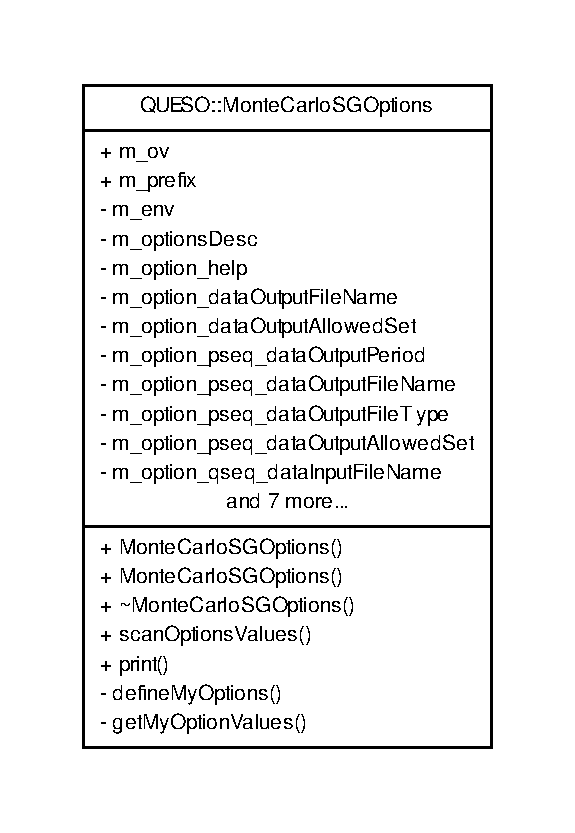
\includegraphics[trim={0.5cm 1.3cm 0 0},clip,scale=0.7]{rawfigs/monte_carlo_options}\label{fig-monte-carlo-options-class}}
\vspace*{-.2cm}
\caption{The Monte Carlo sequence generator class and the Monte Carlo sequence generator options class.}
\end{figure}



\begin{table}[htpb]
% from uqMonteCarloSGOptions.C and uqMonteCarloSGOptions.h
\begin{center}
\caption{Input file options for a QUESO statistical forward problem solved via Monte Carlo algorithm.}
\vspace{-8pt}
\label{tab-monte-carlo-options}
\ttfamily\footnotesize
\begin{tabular}{l c  m{6cm}}
\toprule
\rmfamily Option Name     & \rmfamily Default Value \\
\midrule\midrule
\textlangle PREFIX\textrangle mc\_dataOutputFileName           &  "."  \\
\textlangle PREFIX\textrangle mc\_dataOutputAllowedSet         &       \\
\textlangle PREFIX\textrangle mc\_pseq\_dataOutputFileName     &  "."  \\
\textlangle PREFIX\textrangle mc\_pseq\_dataOutputAllowedSet   &       \\
\textlangle PREFIX\textrangle mc\_qseq\_dataInputFileName      &  "."  \\
\textlangle PREFIX\textrangle mc\_qseq\_size                   &  100  \\
\textlangle PREFIX\textrangle mc\_qseq\_displayPeriod          &  500  \\  
\textlangle PREFIX\textrangle mc\_qseq\_measureRunTimes        &    0  \\  
\textlangle PREFIX\textrangle mc\_qseq\_dataOutputFileName     &  "."  \\ 
\textlangle PREFIX\textrangle mc\_qseq\_dataOutputAllowedSet   &       \\  
\bottomrule
\end{tabular}
\end{center}
\end{table}

% 
% \begin{table}[htpb]
% % from uqMonteCarloSGOptions.C and uqMonteCarloSGOptions.h
% \begin{center}
% \caption{Input file options for a QUESO statistical forward problem solved via Monte Carlo algorithm.}
% \vspace{-8pt}
% \label{tab-monte-carlo-options}
% \ttfamily
% \begin{tabular}{l c  m{6cm}}
% \toprule
% \rmfamily Option Name     & \rmfamily Default Value &  \rmfamily Description \\ %
% \midrule\midrule
% %\textlangle PREFIX\textrangle mc\_help                        &         &             \\ %_ODV = option default value
% %\hline
% \textlangle PREFIX\textrangle mc\_dataOutputFileName           &   "."   &             \\ % m_dataOutputFileName         (UQ_MOC_SG_DATA_OUTPUT_FILE_NAME_ODV 
% %\hline
% \textlangle PREFIX\textrangle mc\_dataOutputAllowedSet         &         &             \\ %//m_dataOutputAllowedSet       (),
% %\hline
% \textlangle PREFIX\textrangle mc\_pseq\_dataOutputFileName     &    "."  &             \\ %m_pseqDataOutputFileName     (UQ_MOC_SG_PSEQ_DATA_OUTPUT_FILE_NAME_ODV
% %\hline
% \textlangle PREFIX\textrangle mc\_pseq\_dataOutputAllowedSet   &         &             \\ %//m_pseqDataOutputAllowedSet   (),
% %\hline
% %\textlangle PREFIX\textrangle mc\_pseq\_computeStats           &         &             \\ %
% % \hline
% \textlangle PREFIX\textrangle mc\_qseq\_dataInputFileName      &   "."   &             \\ %m_qseqDataInputFileName      (UQ_MOC_SG_QSEQ_DATA_INPUT_FILE_NAME_ODV ),
% % \hline
% \textlangle PREFIX\textrangle mc\_qseq\_size                   &   100   &             \\ %m_qseqSize                   (UQ_MOC_SG_QSEQ_SIZE_ODV
% % \hline
% \textlangle PREFIX\textrangle mc\_qseq\_displayPeriod          &  500    &             \\ %m_qseqDisplayPeriod          (UQ_MOC_SG_QSEQ_DISPLAY_PERIOD_ODV
% % \hline
% \textlangle PREFIX\textrangle mc\_qseq\_measureRunTimes        &    0    &             \\ %m_qseqMeasureRunTimes        (UQ_MOC_SG_QSEQ_MEASURE_RUN_TIMES_ODV
% % \hline
% \textlangle PREFIX\textrangle mc\_qseq\_dataOutputFileName     &   "."   &             \\ %m_qseqDataOutputFileName     (UQ_MOC_SG_QSEQ_DATA_OUTPUT_FILE_NAME_ODV),
% % \hline
% \textlangle PREFIX\textrangle mc\_qseq\_dataOutputAllowedSet   &         &             \\ %//m_qseqDataOutputAllowedSet   (),
% % \hline
% %\textlangle PREFIX\textrangle mc\_qseq\_computeStats           &         &             \\ %
% \bottomrule
% \end{tabular}
% \end{center}
% \end{table}



% %\clearpage
% \subsection{Options for Statistical Analysis of Sequences}
% 
% \begin{figure}[htpb]
% \centering
% \includegraphics[scale=0.40,clip=true]{figs/uqSequenceStatisticalOptions}
% \vspace*{-8pt}
% \caption{{\color{red}{The sequence statistical options class}}.}
% \label{fig-seq-statistical-options-class}
% \end{figure}
% 
% \begin{table}[htpb]
% \begin{center}
% \caption{Input file options for a the statistical analysis of sequences.}
% \ttfamily
% \begin{tabular}{l|c|c}
% \toprule
% \rmfamily Option Name  & \rmfamily Default Value & \rmfamily Description \\
% \midrule\midrule
% \textlangle PREFIX\textrangle stats\_help                      &         &             \\
% % \hline
% \textlangle PREFIX\textrangle stats\_initialDiscardedPortions  &         &             \\
% % \hline
% \hline
% \textlangle PREFIX\textrangle stats\_bmm\_run                   &         &             \\
% % \hline
% \textlangle PREFIX\textrangle stats\_bmm\_lengths               &         &             \\
% % \hline
% \textlangle PREFIX\textrangle stats\_bmm\_display               &         &             \\
% % \hline
% \textlangle PREFIX\textrangle stats\_bmm\_write                 &         &             \\
% % \hline
% \hline
% \textlangle PREFIX\textrangle stats\_fft\_compute               &         &             \\
% % \hline
% \textlangle PREFIX\textrangle stats\_fft\_paramId               &         &             \\
% % \hline
% \textlangle PREFIX\textrangle stats\_fft\_size                  &         &             \\
% % \hline
% \textlangle PREFIX\textrangle stats\_fft\_testInversion         &         &             \\
% % \hline
% \textlangle PREFIX\textrangle stats\_fft\_write                 &         &             \\
% % \hline
% \hline
% \textlangle PREFIX\textrangle stats\_psd\_compute               &         &             \\
% % \hline
% \textlangle PREFIX\textrangle stats\_psd\_numBlocks             &         &             \\
% % \hline
% \textlangle PREFIX\textrangle stats\_psd\_hopSizeRatio          &         &             \\
% % \hline
% \textlangle PREFIX\textrangle stats\_psd\_paramId               &         &             \\
% % \hline
% \textlangle PREFIX\textrangle stats\_psd\_write                 &         &             \\
% % \hline
% \hline
% \textlangle PREFIX\textrangle stats\_psdAtZero\_compute         &         &             \\
% % \hline
% \textlangle PREFIX\textrangle stats\_psdAtZero\_numBlocks       &         &             \\
% % \hline
% \textlangle PREFIX\textrangle stats\_psdAtZero\_hopSizeRatio    &         &             \\
% % \hline
% \textlangle PREFIX\textrangle stats\_psdAtZero\_display         &         &             \\
% % \hline
% \textlangle PREFIX\textrangle stats\_psdAtZero\_write           &         &             \\
% % \hline
% \hline
% \textlangle PREFIX\textrangle stats\_geweke\_compute            &         &             \\
% % \hline
% \textlangle PREFIX\textrangle stats\_geweke\_naRatio            &         &             \\
% % \hline
% \textlangle PREFIX\textrangle stats\_geweke\_nbRatio            &         &             \\
% % \hline
% \textlangle PREFIX\textrangle stats\_geweke\_display            &         &             \\
% % \hline
% \textlangle PREFIX\textrangle stats\_geweke\_write              &         &             \\
% % \hline
% \hline
% \textlangle PREFIX\textrangle stats\_autoCorr\_computeViaDef    &         &             \\
% % \hline
% \textlangle PREFIX\textrangle stats\_autoCorr\_computeViaFft    &         &             \\
% % \hline
% \textlangle PREFIX\textrangle stats\_autoCorr\_secondLag        &         &             \\
% % \hline
% \textlangle PREFIX\textrangle stats\_autoCorr\_lagSpacing       &         &             \\
% % \hline
% \textlangle PREFIX\textrangle stats\_autoCorr\_numLags          &         &             \\
% % \hline
% \textlangle PREFIX\textrangle stats\_autoCorr\_display          &         &             \\
% % \hline
% \textlangle PREFIX\textrangle stats\_autoCorr\_write            &         &             \\
% % \hline
% \hline
% \textlangle PREFIX\textrangle stats\_meanStacc\_compute         &         &             \\
% % \hline
% \hline
% \textlangle PREFIX\textrangle stats\_hist\_compute              &         &             \\
% % \hline
% \textlangle PREFIX\textrangle stats\_hist\_numInternalBins      &         &             \\
% % \hline
% \hline
% \textlangle PREFIX\textrangle stats\_cdfStacc\_compute          &         &             \\
% % \hline
% \textlangle PREFIX\textrangle stats\_cdfStacc\_numEvalPositions &         &             \\
% % \hline
% \hline
% \textlangle PREFIX\textrangle stats\_kde\_compute               &         &             \\
% % \hline
% \textlangle PREFIX\textrangle stats\_kde\_numEvalPositions      &         &             \\
% % \hline
% \hline
% \textlangle PREFIX\textrangle stats\_covMatrix\_compute         &         &             \\
% % \hline
% \textlangle PREFIX\textrangle stats\_corrMatrix\_compute        &         &             \\
% \bottomrule
% \end{tabular}
% \end{center}
% \label{tab-seq-statistical-options}
% \end{table}
% 

%\clearpage
\section{Miscellaneous Classes and Routines}
 
As the name suggests, QUESO miscellaneous classes and routines have a variety of routines.
For instance, the function \verb+MiscReadDoublesFromString+ is used for reading the options input files and assigning the values to the respective variables, in \texttt{uqMonteCarloSGOptions::} \texttt{getMyOptionValues} and in \verb+MetropolisHastingsSGOptions::getMyOptionValues+. 

QUESO class \verb+BaseOneDGrid+ generates grids necessary for calculating the CDF of a RV; it is required by class \verb+ArrayOfOneDGrids+, which, in turn, is used in both classes: \linebreak \verb+StatisticalForwardProblem+ and \verb+StatisticalInverseProblem+.

% %\clearpage
% \section{Interface Classes}
% 
% \todo{Define what `interface' means here. Is is interface to C and Fortran? }
% /src/interface/basic...
% 
% \subsection{Using Other C++ Classes in the Library}
% 
% https://svn.ices.utexas.edu/repos/pecos/turbulence/IncompRansCal/calDataLevModUncert/README


% \subsection{Input and Output Files}

